
%% The following is a directive for TeXShop to indicate the main file
%%!TEX root = ../../thesis.tex

\chapter{An inversion approach for subsurface injections}
\label{ch:inversion}

\section{Introduction}

The previous three chapters have focussed on understanding the physics of electromagnetics over conductive, permeable, steel-cased wells. In this chapter, we return to the goal of imaging subsurface injections through geophysical inversion. We view this as a time-lapse problem, in which one data set is obtained prior to the injection and second data set is obtained after the injection. The aim of the inversion, then, is to characterize the changes in the earth model due to the injection.

Time-lapse direct current (DC) resistivity, and in some cases electromagnetics (EM), is commonly used in the groundwater hydrology community. In particular, DC resistivity has been used, in salt-tracer experiments aimed at understanding groundwater flow (e.g. \cite{Slater2002, Kemna2002, Singha2005, Doetsch2012}) and for characterizing time-lapse vadose zone processes (e.g. \cite{Daily1992, Park1998, Binley2002}). Within the context of hydrogeophysics, typically multiple time-lapse surveys are conducted. A range of interpretation techniques have been applied. In terms of algorithmic complexity, the most straightforward approach is to invert each time-snapshot independently. The recovered models can then be differenced and the difference interpreted \citep{Cassiani2006}, or an intermediate interpretation, for example estimating the center of mass of a plume \citep{Singha2006, Doetsch2012}, can serve as an indicator that is tracked through time. \cite{Daily1992} presented an approach for inverting ratios between initial and subsequent datasets, and \citep{Labreque2001} proposed an inversion for the resistivity difference between two subsequent data sets by inverting the difference between the two data sets. A common approach is to use the inversion result from an initial timestep as a reference and starting model for the following datasets \citep{Loke2001, Oldenborger2007}, this is sometimes referred to as a ``cascaded inversion'' \citep{Miller2008}. More advanced techniques simultaneously invert all of the time-snapshots and apply both spatial and temporal regularization \citep{Kim2009, Kim2010, Loke2014}. \cite{Hayley2011} provides an overview and comparison of common time-lapse inversion approaches and demonstrates a comparison of several approaches for a synthetic example of the remediation of a saline plume.

In the context of reservoir imaging applications, the ``time-lapse'' aspect of the problem is somewhat simpler than that typically encountered in hydrogeophysics. Very few temporally-dense DC or EM data sets have been collected for reservoir imaging. Notable exceptions include the cross-well DC resistivity surveys described in \cite{Carrigan2013} and \cite{Tondel2014}, for monitoring of a deep CO$_2$ injection in a gas field and monitoring steam chamber growth in a steam-assisted gravity drainage operation in the Athabasca Oil sands, respectively. Much more common are time-lapse data sets consisting of only two times: pre-injection and post-injection. Cross-well EM has been applied for such surveys in to monitor water-floods \citep{Wilt2005, Wilt2012} and steam injections \citep{Wilt1996, Wilt1997, Marion2011}. By far, the most common inversion approach involves inverting for a background model with the initial data set, typically including constraints from well-logs and potentially interfaces from seismic data and using this as the starting model for the inversion, typically in 2D (e.g. \cite{Wilt2012}).

Although the ``time-lapse'' aspect of injection-monitoring applications is generally simpler than applications in hydrogeophysics, the large depths considered in reservoir applications means that we are usually working with small signals. Furthermore, the presence of steel cased wells complicates signals. Efforts to reduce the impact of steel cased wells on DC surveys include using a coating on the casing which the electrodes are connected to insulate the casing from the survey \citep{Tondel2014}. For cross-well EM applications, fibreglass casings may sometimes be used \citep{Wilt2012}, or when a single well is cased, a ``casing-correction'' is applied to the data collected at a fixed frequency \citep{Wu1993}.

For the emerging application of grounded-source DC or EM in the monitoring of subsurface injections, very few inversions of synthetic or field studies have been published and there are many open questions. How does the casing affect our sensitivities in the inversion? In particular, \cite{}, have shown that in near surface studies, where … and forward modelling shows that the currents spread out along the length of the well, can we expect to resolve the location of the target along the well? Specific to subsurface injections, there is also further a-priori information that may be included, for example the conductivity of the injected material and the volume of material injected can be considered know. How best do we include this information in the inversion?

To focus discussion, we will consider synthetic examples related to hydraulic fracturing. The goal of the inversion in this case is to delineate the extent and geometry of the propped region of the fractured reservoir. Changes in electrical conductivity are viewed as a proxy for estimating the concentration of propped fractures.


We will consider voxel based, parametric
alternative model parameterizations using effective medium theory

Incorporate volume information about the subsurface injection

Notebooks are available at https://github.com/simpeg-research/heagy-2018-injection-inversions


\section{Geophysical Inversions}
In this section, we provide a brief overview of geophysical inversions, adapted from \cite{Cockett2015}; for more detail and examples, the reader is reffered to \cite{Oldenburg2005, Cockett2015} as well as Appendix \ref{ch:simpegem} for details specific to forward and inverse modelling in electromagnetics.

The aim of a geophysical inversion is to use the collected data to extract information about the subsurface. In a given survey, a datum can be written as

\begin{equation}
F_i[\mathbf{m}] + \epsilon_i = d_i
\label{eq:geophysical_datum}
\end{equation}

where $F[\cdot]$ is the forward simulation operator; for an electromagnetic problem, it simulates Maxwell’s equations given a source and samples the relevant fields and fluxes at the receiver locations. The physical properties of the subsurface are captured by the variable $m$, which we refer to as the inversion model. The noise is described by $\epsilon_i$, and $d_i$ is the observed datum. A survey usually includes multiple sources and receivers, resulting in the observed data $\mathbf{d}_{\rm obs} = [d_1, ... , d_N]$ and some estimate of their uncertainties -- often assumed to be Gaussian. If the noise is Gaussian, then an appropriate measure of the data misfit is the $l_2$-norm of the difference between the predicted data obtained through a forward simulation and the observed data, namely

\begin{equation}
\phi_{\rm d}(\mathbf{m}) = \frac{1}{2}\|\mathbf{W}_{\rm d}(F[\mathbf{m}] - \mathbf{d}_{\rm obs})\|^2
\label{eq:data_misfit}
\end{equation}

$\mathbf{W}_{\rm d}$ is a diagonal matrix whose elements are equal to $\mathbf{W}_{\rm d_{ii}}=1/\epsilon_i$ where $\epsilon_i$ is an estimated standard deviation of the $i$\textsuperscript{th} datum. A good option is to assign a $\epsilon_i = floor + \%|d_i|$.
Percentages are generally required when there is a large dynamic range of the data. A percentage alone can cause great difficulty for the inversion if a particular datum acquires a value close to zero, and therefore we include a floor.

In addition to a metric that evaluates the size of the misfit, it is also required that we have a tolerance, $\phi_d^*$; models satisfying $\phi_d(\mathbf{m}) \leq \phi_d^*$ are considered to adequately fit the data \citep{Parker1994}. If the data errors are Gaussian and we have assigned the correct standard deviations, then the expected value of $\phi_d^* \sim N/2$, where $N$ is the number of data. Finding a model that has a misfit substantially lower than this will result in a solution that has excessive and erroneous structure, that is, we are fitting the noise. Finding a model that has a misfit substantially larger than this will yield a model that is missing structure that could have been extracted from the data (see \cite{Oldenburg2005} for a tutorial).

The goal of an inversion is to estimate the earth-model, $m$ from the data. In reality, the physical property distribution of the subsurface is continuous; therefore, estimating this model from a finite number of data is an ill-posed problem, meaning no unique model explains the data. Thus, in order to obtain a meaningful model from the data, assumptions and additional information must be included. There are several mechanisms by which this can be achieved. One of the most common is to include consideration of a model regularization, $\phi_m$ in the inverse problem. This norm can penalize variation from a reference model, spatial derivatives of the model, or some combination of these. For example, the Tikhonov-style regularization function can be expressed as

\begin{equation}
\phi_{\rm m}(\mathbf{m}) =
    \frac{\alpha_s}{2}\|\mathbf{W}_{\rm s}(\mathbf{m} - \mathbf{m}_{\rm ref})\|^2 +
    \frac{\alpha_x}{2}\|\mathbf{W}_{\rm x}\mathbf{m}\|^2 +
    \frac{\alpha_y}{2}\|\mathbf{W}_{\rm y}\mathbf{m}\|^2 +
    \frac{\alpha_z}{2}\|\mathbf{W}_{\rm z}\mathbf{m}\|^2
\label{eq:model_regularization}
\end{equation}

The first term is referred to as the ``smallness'' and penalizes difference between the inversion model and a reference model $\mathbf{m_{\rm ref}}$. The matrix $\mathbf{W}_s$ is a diagonal matrix; in the simplest case it is the identity matrix. The remaining three terms are the first-order smoothness in the x, y, and z directions; the matrices $\mathbf{W}_{\rm x}$, $\mathbf{W}_{\rm x}$, $\mathbf{W}_{\rm y}$ and $\mathbf{W}_{\rm z}$ approximate the first order spatial derivatives in each direction. The $\alpha$ parameters weight the relative contribution of each term to the regularization. Their values should consider the length-scales in the problem (c.f. \cite{Oldenburg2005}); for a typical 3D problem $\alpha_x = \alpha_y = \alpha_z = 1$ and $\alpha_s$ is generally chosen to be several orders of magnitude smaller than the smoothness weights.

To define the inverse problem, we take a deterministic approach to the inversion and treat the it as an optimization problem. Additional strong constraints on the model such as upper and lower bounds ($\mathbf{m}_u$, $\mathbf{m}_l$) are also considered. The general form of the objective function we use combines the data misfit and regularization with a trade-off parameter, $\beta$, between them, giving a problem of the form

\begin{equation}
\begin{split}
&\underset{\mathbf{m}}{\text{minimize}} \quad \phi(\mathbf{m}) = \phi_d(\mathbf{m}) + \beta \phi_m(\mathbf{m}) \\
&\text{such that} \quad \phi_d \leq \phi_d^*, \quad \mathbf{m}_l \leq \mathbf{m} \leq \mathbf{m}_u
\end{split}
\label{eq:inverse_problem}
\end{equation}

Since the value of $\beta$ is not known \emph{a priori}, the above optimization problem can be solved at many values of $\beta$ to produce a trade-off, or Tikhonov, curve (cf. \cite{Parker1994}). An optimum value, $\beta^*$, can be found so that solving equation \ref{eq:inverse_problem} with $\beta^*$ produces a model with misfit $\phi_d^*$. One approach to finding the value of $\beta^*$ is to use cooling techniques where the $\beta$ is progressively reduced from some high value and the process stopped when the tolerance is reached.

The optimization problem posed equation \ref{eq:inverse_problem} is non-linear for DC resistivity and electromagnetic forward simulations requiring that iterative optimization techniques be employed (c.f. \cite{Nocedal1999}). Gradient-based techniques are commonly employed. In particular, Gauss-Newton methods are effective in geophysical inversions. To ease notation, we consider a more compact description of the model regularization, and write our objective function as

\begin{equation}
\phi(\mathbf{m}) = \frac{1}{2}\|\mathbf{W}_{\rm d}(F[\mathbf{m}] - \mathbf{d}_{\rm obs})\|^2 + \frac{\beta}{2}\|\mathbf{W}_{\rm m}\mathbf{m}\|^2
\label{eq:objective_function}
\end{equation}

Note that if $\mathbf{m}_{\rm ref} = \mathbf{0}$ and $\mathbf{W}_{\rm m} = [\mathbf{W}_{\rm s}^\top, \mathbf{W}_{\rm x}^\top, \mathbf{W}_{\rm y}^\top, \mathbf{W}_{\rm z}^\top]^\top$, then the regularization is equivalent to that stated in equation \ref{eq:model_regularization}. The gradient is given by

\begin{equation}
\mathbf{g}(\mathbf{m})=
    J[\mathbf{m}]^\top \mathbf{W}_{\rm d}^\top \mathbf{W}_{\rm d}(F[\mathbf{m}]-\mathbf{d}_{\rm obs})
    + \beta \mathbf{W}_{\rm m}^\top \mathbf{W}_{\rm m} (\mathbf{m})
\label{eq:objective_function_gradient}
\end{equation}

where $J[\mathbf{m}]$ is the sensitivity or Jacobian. The components $J[\mathbf{m}]_{ij}$ specify how the $i$\textsuperscript{th} datum changes with respect to the $j$\textsuperscript{th} model parameter,

\begin{equation}
    J[\mathbf{m}] = \frac{d F[\mathbf{m}]}{d \mathbf{m}}
\label{eq:sensitivity}
\end{equation}

We discuss the derivation of the sensitivity for time and frequency domain electromagnetic problems in depth in Appendix \ref{ch:simpegem}.

At the $k$\textsuperscript{th} iteration, beginning with a model $\mathbf{m}^{k}$, we search for a perturbation $\delta \m$ that reduces the objective function. Linearizing the forward simulation by Taylor expansion,

\begin{equation}
F[\mathbf{m}^{k}+\delta \mathbf{m}] \simeq F[\mathbf{m}^{k}] + \mathbf{J}[\mathbf{m}^{k}]\delta \mathbf{m} + \mathcal{O}(\delta \mathbf{m})^2
\label{eq:taylor_expand_forward_simulation}
\end{equation}


and setting the gradient equal to zero yields the standard Gauss-Newton equations
to be solved for the perturbation $\delta \mathbf{m}$:

\begin{equation}
(J[\mathbf{m}]^\top \mathbf{W}_{\rm d}^\top \mathbf{W}_{\rm d} J[\mathbf{m}] + \beta \mathbf{W}_{\rm m}^\top \mathbf{W}_{\rm m}) \delta \mathbf{m} = -\mathbf{g}(\mathbf{m})
\label{eq:gauss_newton}
\end{equation}

The updated model is given by

\begin{equation}
\mathbf{m}^{k+1}=\mathbf{m}^{k} + \gamma \delta \mathbf{m}
\label{eq:model_update}
\end{equation}

where $\gamma \in (0,1]$ is a coefficient that can be found by a line search.
Setting $\gamma=1$ is the default and a line search is necessary if $\phi(\mathbf{m}^{k+1}) \ge \phi(\mathbf{m}^{k})$.

The iterative optimization process is continued until a suitable stopping criterion is reached.
Completion of this iterative process yields a minimization for particular value of the trade-off parameter, $\beta$. If we are invoking a cooling schedule, and if the desired misfit tolerance is not yet achieved, $\beta$ is reduced and the iterative numerical optimization procedure is repeated.

The forward simulation, computation of the sensitivities, and inversion machinery that we use throughout this chapter are implemented in the open source software package, \texttt{SimPEG} \citep{Cockett2015, Heagy2017}.
\subsection{Choosing an inversion model}
At this stage, we have laid out a strategy for inverting for the inversion model $\mathbf{m}$, but we have yet to specify how we define $\mathbf{m}$. The physical property to which aim to characterize in an electromagnetic inversion is electrical conductivity $\sigma$ (or equivalently, its inverse, resistivity $\rho$). In a DC or an EM inversion, however, it is common to invert for log-conductivity on the forward simulation mesh, that is

\begin{equation}
\sigma = \mathcal{M}(\mathbf{m})
\label{eq:mapping}
\end{equation}

where $\mathcal(\mathbf{m}) = \exp{\mathbf{m}}$. We refer to $\mathcal{M}(\cdot)$ as a mapping. Mappings have two implications in the inversion. One implication is in the model regularization: we have changed the space in which we are applying the regularization, for this example, we regularize on log-conductivity values rather than linear conductivity. As the conductivity of common earth materials varies over several orders of magnitude, it is preferable to penalize jumps in orders of magnitude between voxels rather than penalizing linear values. The second implication is in the computation of the sensitivity. The forward simulation in an EM or DC problem depends upon electrical conductivity, thus the mapping modifies the sensitivity via the chain rule

\begin{equation}
    J[\mathbf{m}] = \frac{d F[\mathcal{M}(\mathbf{m})]}{d \mathcal{M}(\mathbf{m})}\frac{d \mathcal{M}(\mathbf{m})}{d \mathbf{m}} = \frac{d F[\sigma(\mathbf{m})]}{d \sigma}\frac{d \sigma}{d \mathbf{m}}
\label{eq:sensitivity_mappings}
\end{equation}


Mappings can be composed, for example if inactive cells are included in the modelling domain, such as air cells or cells capturing known structures such as a steel-cased well, then

\begin{equation}
\sigma = \mathcal{M}_2(\mathcal{M}_1(\mathbf{m}))
\label{eq:compose_mappings}
\end{equation}

where $\mathcal{M}_1$ injects in the log-conductivity values of the inactive cells and $\mathcal{M}_2$ takes the exponential. The sensitivity is appropriately modified by adding another step to the chain rule.

In addition to mappings routinely employed in electromagnetic inversions, such as those used for working with log-conductivity values and handling inactive cells in the modelling domain, there are two mapping which we will make use of in this chapter: an effective medium theory mapping, based on the homogenization technique for propped, fractured reservoirs discussed in chapter \ref{ch:phys_prop_model} and parametric mappings.

\subsubsection{Parametric mappings}

The other type of mapping will make extensive use of in this chapter are parametric maps. We consider the model parameterizations of blocks and ellipsoids, similar to that described in \cite{McMillan2015a, Mcmillan2017}. For example, using a simple parametrization of a block, the model is

\begin{equation}
\mathbf{m} = [m_{\rm back}, m_{\rm block}, x_0, \Delta x, y_0, \Delta y, z_0, \Delta z]^\top
\label{eq:model_block}
\end{equation}

where $m_{\rm back}$ is the model value of the background, $m_{\rm block}$, $(x_0, y_0, z_0)$ is the center of the block and ($\Delta x, \Delta y, \Delta z$) are the widths of the block in each dimension. The mapping is then

\begin{equation}
\mathcal{M}(\mathbf{m}) =
    m_{\rm back} +
    (m_{\rm block} - m_{\rm back})~s(\tau(\mathbf{m}))
\label{eq:mapping_block}
\end{equation}

where $s(\cdot)$ is a differentiable approximation to a step-function and $\tau$ is a level set function of the block. To approximate a step function, we use the arctangent function,

\begin{equation}
s(\tau) = \frac{1}{\pi}\tan^{-1}(a\tau) + \frac{1}{2}
\label{eq:arctan_step}
\end{equation}

where $a$ controls the slope of the transition between 0 and 1. Small values of $a$ result in a gradual transition while larger values give a sharper transition. For more robust performance of the Gauss-Newton inversion, we choose $a$ such that the transition happens over a multiple cells in the simulation mesh \citep{Mcmillan2017}.

A block is defined by the infinity norm,

\begin{equation}
\tau = 1 - \left(
    \left|\left|\frac{x - x_0}{\Delta x / 2}\right|\right|_\infty^2 +
    \left|\left|\frac{y - y_0}{\Delta y / 2}\right|\right|_\infty^2 +
    \left|\left|\frac{z - z_0}{\Delta z / 2}\right|\right|_\infty^2
\right)
\label{eq:tau_infinity}
\end{equation}

however the infinity norm is not differentiable. Thus, we approximate the infinity norm using an ekblom norm

\begin{equation}
\tau = 1 - \left(
    \left[\left(\frac{x - x_0}{\Delta x / 2}\right)^2 + \varepsilon^2 \right]^{p/2} +
    \left[\left(\frac{y - y_0}{\Delta y / 2}\right)^2 + \varepsilon^2 \right]^{p/2} +
    \left[\left(\frac{z - z_0}{\Delta z / 2}\right)^2 + \varepsilon^2 \right]^{p/2}
\right)
\label{eq:tau_ekblom}
\end{equation}

where $\varepsilon$ is a small constant and $p$ is a constant describing the approximate norm, for example, if $p=2$, then equation \ref{eq:tau_ekblom} describes an ellipsoid. To represent a block, we choose a $p$ that is sufficiently large. For the length scales we consider, a value of $p=4$ is appropriate. The value of $\varepsilon$ is chosen to be large enough, and the value of $p$ small enough so that that the derivatives of the mapping are stable and second-order for the length scales of the problem. In addition, rotations can be included in the model, as described in \cite{Mcmillan2017} \footnote{\cite{Mcmillan2017} also employs a weighting scheme to scale the model parameters. We have not found this to be necessary for the examples we consider and thus do not use any weights or scaling}.

When employing parametric mappings, there are two important implications to note in the setup of the inversion. Since the mathematical statement of the inverse problem is overdetermined, there are more data than model parameters, we fix the value of $\beta$ at zero and do not employ a regularization. The second point is that for a starting model, it is important to start with the block and background having different conductivities. This was similarly discussed in \cite{Mcmillan2017}.

\subsubsection{Effective medium theory mapping}

In chapter \ref{ch:phys_prop_model}, we introduced a two-step process for estimating the electrical conductivity of a propped, fractured volume of rock. The first step involved estimating the effective conductivity of a mixture of electrically conductive proppant and fluid, and in the second step, we estimated the effective conductivity of a volume of rock which has fractures filled with the proppant-fluid composite.

Assuming the electrical conductivity of the fluid and proppant are known, then rather than inverting for electrical conductivity, we can invert for the concentration of conductive fractures. To avoid introducing additional non-uniqueness into the problem, we use a fixed ratio of proppant and fluid in within the propped region of the reservoir and treat the fracture concentration $\varphi$ as the inversion model. In a voxel-based inversion, $\varphi$ is a vector with a value for the concentration in each cell. For simplicity, we assume that the fractures are randomly oriented and work only with isotropic conductivities. In this case, the mapping requires that we solve the two-pase effective medium theory approximation,

\begin{equation}
    (1-\varphi)(\sigma^* - \sigma_0)R^{(0,*)} + \varphi(\sigma^* - \sigma_1)R^{(1,*)}= 0
\label{eq:effective_medium_theory_mapping}
\end{equation}

for the effective conductivity, $\sigma^*$. The background has conductivity $\sigma_0$ and the conductive, proppant-filled cracks have conductivity $\sigma_1$. Note that $\sigma_0$, the conductivity of the background, does not need to be a scalar, it can be a vector with a background conductivity value for each voxel in the mesh. These values can be obtained by first inverting the pre-fracture data. The electric field concentration tensor $R^{(i,*)}$ captures the geometry of the particles that compose each phase. Note that for randomly oriented fractures $R^{(i,*)}$ is a scalar ($1/3 \text{trace}{\mathbf{R}^{(i,*)}}$, where $\mathbf{R}^{(i,*)}$ is given in equation \ref{eq:emd_r_spheroids}. For the background, we use an aspect ratio of 1, assuming a spherical geometry for the particles that compose it, and for the fractures, we use a small aspect ratio ($\sim 10^{-4} - 10^{-3}$) and treat them as ellipsoidal cracks. In Chapter \ref{ch:phys_prop_model}, we demonstrated that for sufficiently thin fractures, the exact aspect ratio is not significant. For a gradient based inversion, we also require the derivative of the effective conductivity with respect to the fracture concentration; the derivation is outlined in Appendix \ref{app:scemt_derivatives}.

Self-consistent effective medium theory is the method we adopt to connect the concentration of fractures with the effective conductivity of a fractured volume of rock, however, other relationships, such as an empirical relationship estimated from a lab study, could equally be employed. One interesting implication of relating the concentration of the fractures to the change in conductivity is that this provides a conduit for bringing in a-priori information about the volume of proppant injected into the reservoir. The predicted volume is

\begin{equation}
    V_{\rm pred} = \int\varphi ~ dV
\label{eq:predicted_volume}
\end{equation}

We can then define a volume data misfit term,

\begin{equation}
    \phi_V = \frac{1}{2}\left|\left|\frac{1}{\varepsilon_V}(V_{\rm pred} - V_{\rm obs})\right|\right|^2
\label{eq:volume_data_misfit}
\end{equation}

where $V_{\rm obs}$ is the known volume terms which accounts for the estimated ratio of proppant and fluid and $\varepsilon_V$ is an uncertainty term. We note that we are assuming a fixed ratio of proppant and fluid within the cracks. In reality, this will be variable, thus we use an sufficiently large $\varepsilon_V$ as not to over-fit this assumption.

In the implementation the inclusion of an additional data misfit term is handled by a combo-objective function which enables joint inversions in the SimPEG framework.

\section{Inversions with steel-cased wells}

In the Chapter \ref{ch:casing_dc}, we saw that the current spreads out along the length of the casing, decaying as we move away from the source. In the inversion, this raises questions about our ability to resolve the depth and vertical extent of the target. In this section, we start from a simple model of a vertical well with a conductive target and examine our ability to recover that target. Although most fracture operations are conducted in horizontal wells, we start by considering a vertical well as this reduces computational cost and allows us to explore aspects of the behavior of inversion prior to moving to the more fully 3D, more computationally intensive scenario.

We start by considering a DC experiment with a simple cylindrically symmetric model, shown in Figure \ref{fig:DC_cyl_setup}. A 1km long casing is embedded in a background that has a resistivity of of $100$ $\Omega$m. The casing has an outer diameter of 10cm, a thickness of 1 cm and a conductivity of $5 \times 10^6$ S/m. For modelling, we approximate the hollow-cased well as solid cylinder with a conductivity of $1.4 \times 10^4$ S/m, which preserves the product of the conductivity and the cross sectional area. This was shown to be a valid approximation in Chapter \ref{ch:casing_dc} and allows us to reduce the number of cells in the mesh, thus speeding up the computation of the forward simulation and sensitivities. Similar to the model used in \ref{ch:fracture_physprops}, we assume a moderately-sized fracture operation which uses an 800m$^3$ slurry comprised of $15\%$ proppant by volume. We assume leak-off of some of the fluid, leaving a mixture of 50\% fluid and 50\% proppant, by volume, in the fractures. This gives a total fracture volume of 240 m$^3$ which we distribute among 10 each with 3mm width are positioned within a 10m interval along the well. Conserving volume gives a 50m radius for the fractures. Using a fluid conductivity of 3 S/m and a proppant conductivity of 10$^5$ S/m, the conductivity of the 50/50 proppant-fluid mixture found using self-consistent effective medium theory (equation \ref{eq:effective_medium_theory}) is 2500 S/m. Using a fracture aspect ratio of $3 \times 10^{-5}$ and assuming randomly-oriented fractures, we obtain a conductivity of 3 S/m for the propped region of the reservoir.


\begin{figure}
    \begin{center}
    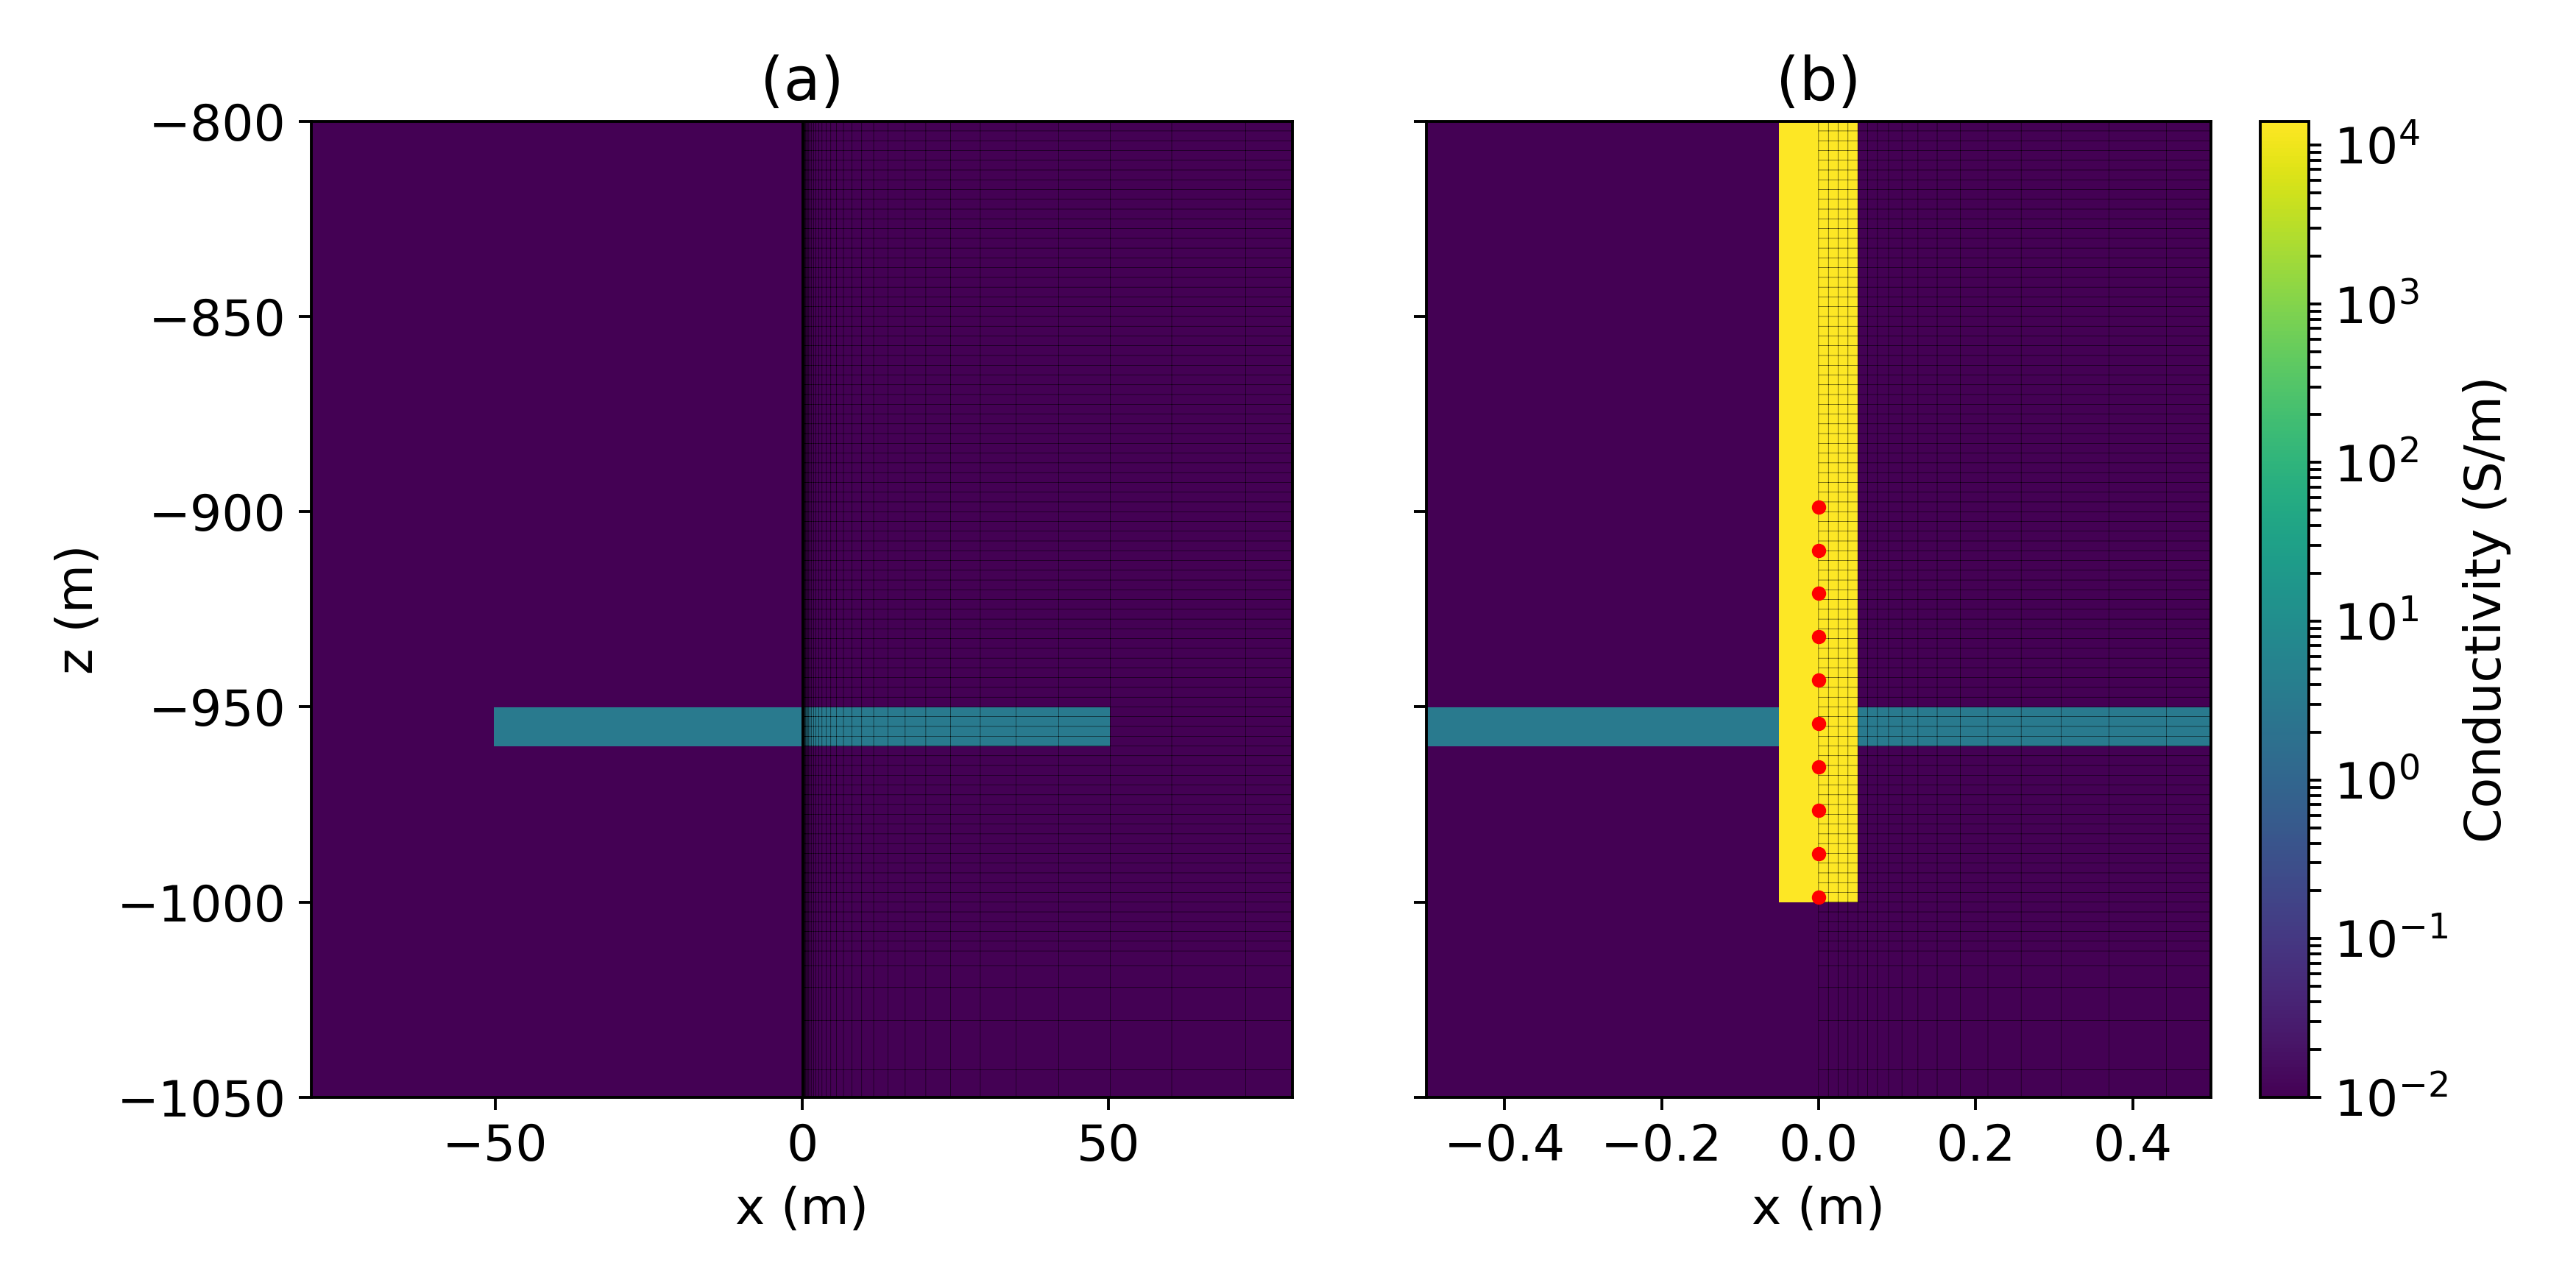
\includegraphics[width=\textwidth]{figures/inversion/DC_cyl_setup.png}
    \end{center}
\caption{
    Model of an electrically conductive propped fracture zone (3 S/m) in a halfspace (100 $\Omega$ m) with a steel-cased well.
    The well is modelled as a solid cylinder with a conductivity of $1.4 \times 10^4$ S/m. The mesh has 4 cells across the
    radius of the casing. The fractured region extends vertically from 950 to 960 m depth and has a radius of 50m.
    Panel (a) has a radial extent of 80 m to show the fractured zone and panel (b) has a radius of 0.4m to show the casing.
    The a-electrode locations are shown in panel (b).
}
\label{fig:DC_cyl_setup}
\end{figure}


The survey we use employs a downhole electrode and a distant return electrode. There are 10 down-hole source locations from 900 m depth to 1000 m depth, as shown by the red dots in Figure \ref{fig:DC_cyl_setup}b. Radial electric field data are collected at the surface; there are 40 receiver locations from 25 m to 1000 m radially away from the well. In total, the survey consists of 400 data. Figure \ref{fig: dc_casing_initial_data} shows the simulated data for both the background (prior to the fracture) and the fracture. The difference between the two is significant both in magnitude and in percentage and thus can expect that the inversion will introduce structure in order to fit the fracture data. In the following sections, we will explore several approaches to the inverse problem for obtaining meaningful information from the data.


\begin{figure}
    \begin{center}
    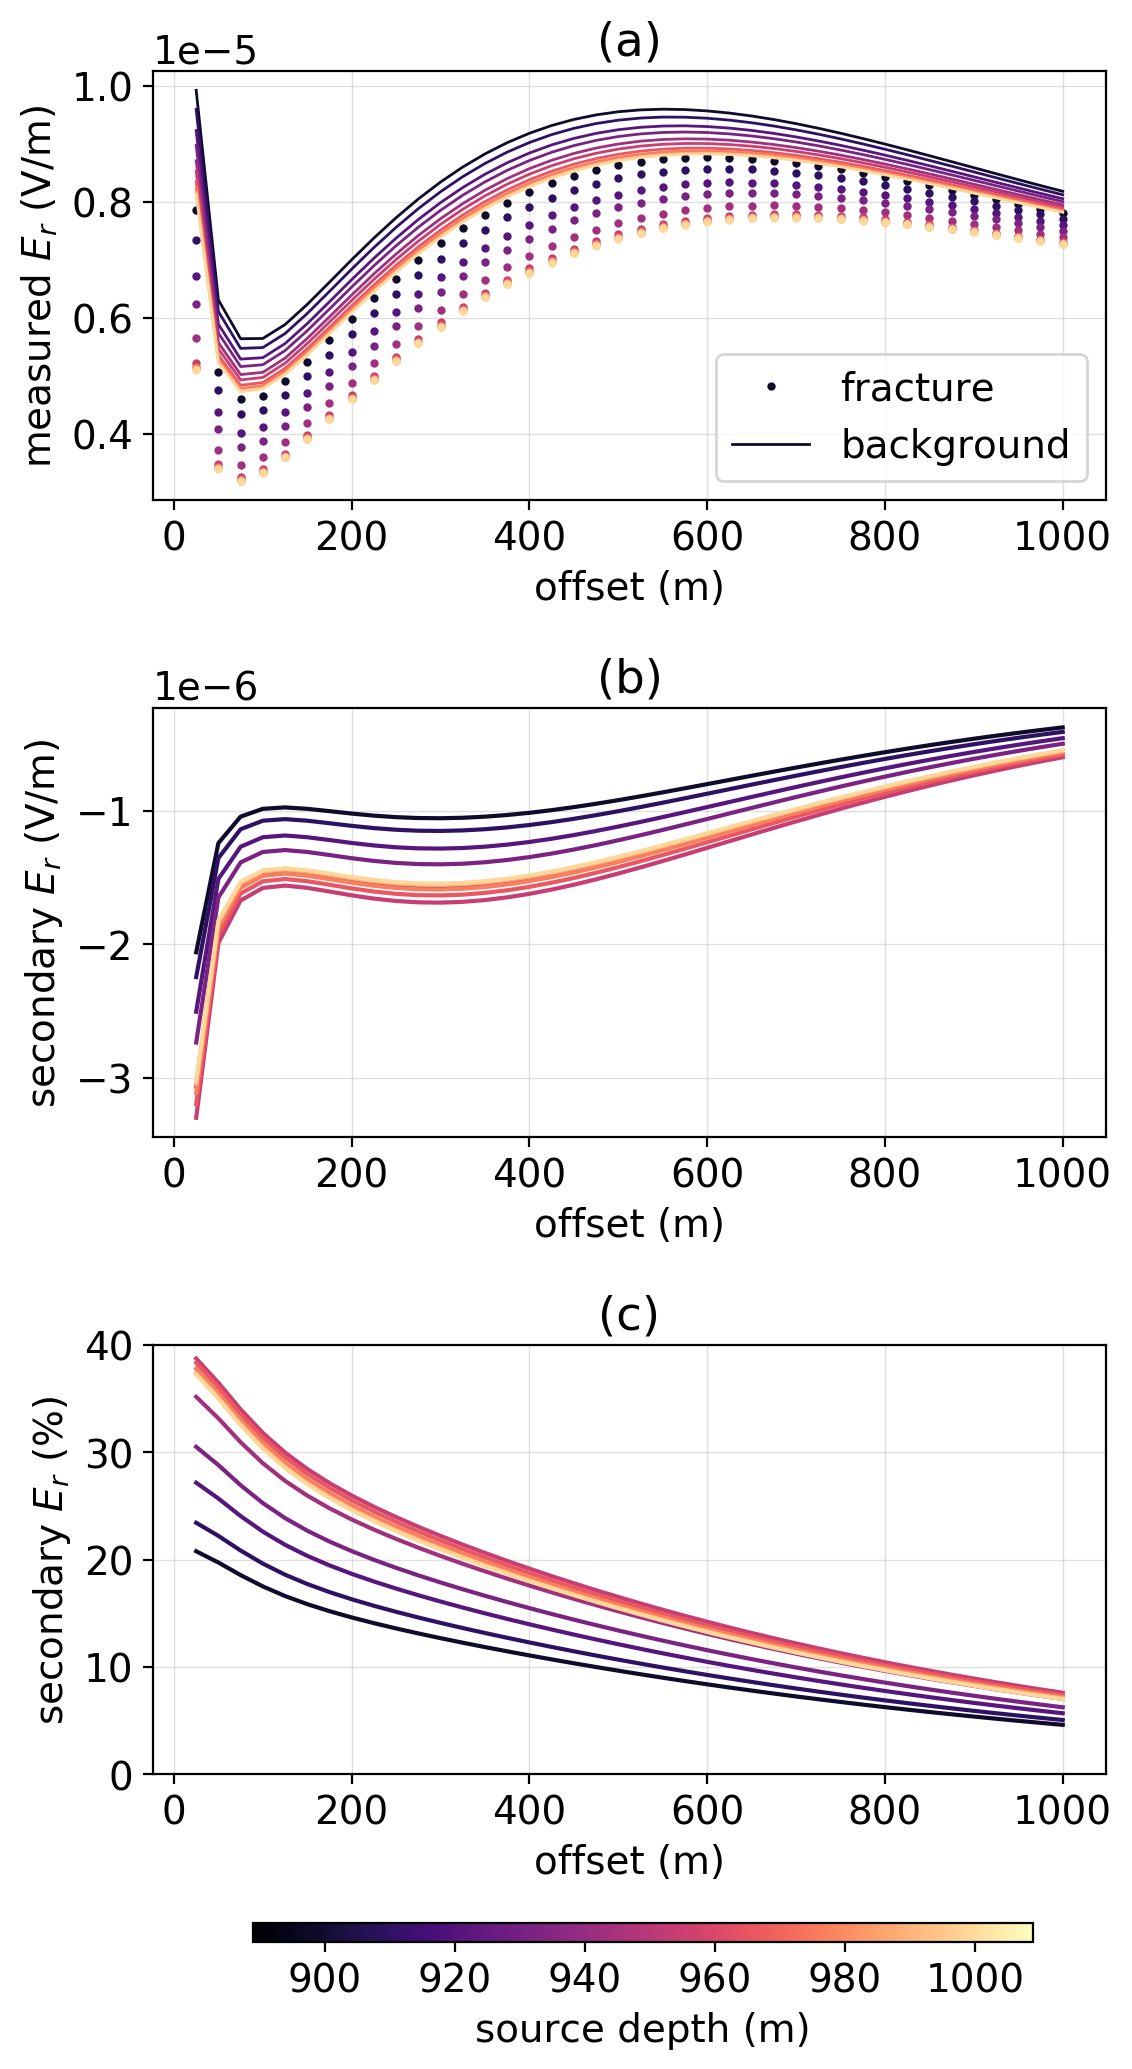
\includegraphics[width=0.6\textwidth]{figures/inversion/dc_casing_initial_data.png}
    \end{center}
\caption{
    (a) Synthetic data for the down-hole casing experiment for the background,
    prior to the fracture (solid lines), and after the fracture (dots), (b) secondary
    electric field (fracture - background), and (c) secondary electric field as a percentage
    of the primary (background). The color of the lines or dots indicates the depth of the source.
}
\label{fig:dc_casing_initial_data}
\end{figure}


\subsection{Standard Tikhonov inversion}
We begin by applying standard inversion techniques and perform a voxel inversion using a Tikhonov regularization. As the simulation is cylindrically symmetric, we invert for a 2D model which varies radially and vertically. Our aim in this inversion and the ones that follow is to examine, under ideal circumstances, what information we can obtain from the data using a given inversion approach. We therefore do not add noise to the data and assign low uncertainties: 1\% with a $10^-9$ V/m floor.

The choice of parameters is quite standard, similar to how one would approach a blind inversion. In the regularization, we use $\alpha_s = 10^{-3}$, $\alpha_x = \alpha_z = 1$. We adopt a $\beta$-cooling schedule that reduces the value of $\beta$ by a factor of 8 every 3 iterations. The initial $\beta$ is chosen by estimating the largest eigenvalue of the  model regularization and data misfit through one iteration of the power method and taking their ratio; $\beta_0$ is then a scalar multiple of that. For the following inversions, we use a factor of 10. The initial and reference model are equal to the half-space resistivity of 100 $\Omega$m.

The results of the first inversion we run are shown in Figure \ref{fig:dc_smooth_inversion_1e-01}. This inversion reached a global $\chi$-factor of $<0.1$ and fits all data points within 5\% (Figure \ref{fig:dc_smooth_inversion_1e-01}c). It converged in two iterations. As expected in an Tikhonov-style inversion, the recovered model is smooth and diffuse. Perhaps unexpected is the location of the center of the recovered target; its depth is shifted below the true location, closer to the end of the well. Typically, we might expect that if the inversion were to shift the location of a target, it would be shifted up, closer to the receivers, where we have greater sensitivity. However, the presence of the casing alters the sensitivity. In Chapter \ref{ch:casing_software}, we demonstrated that there is an increase in charge near the ends of the well (see Figure \ref{fig:kaufman_finite_well}, in particular), for the DC problem, this translates to an increase in sensitivity near the end of the well.


\begin{figure}
    \begin{center}
    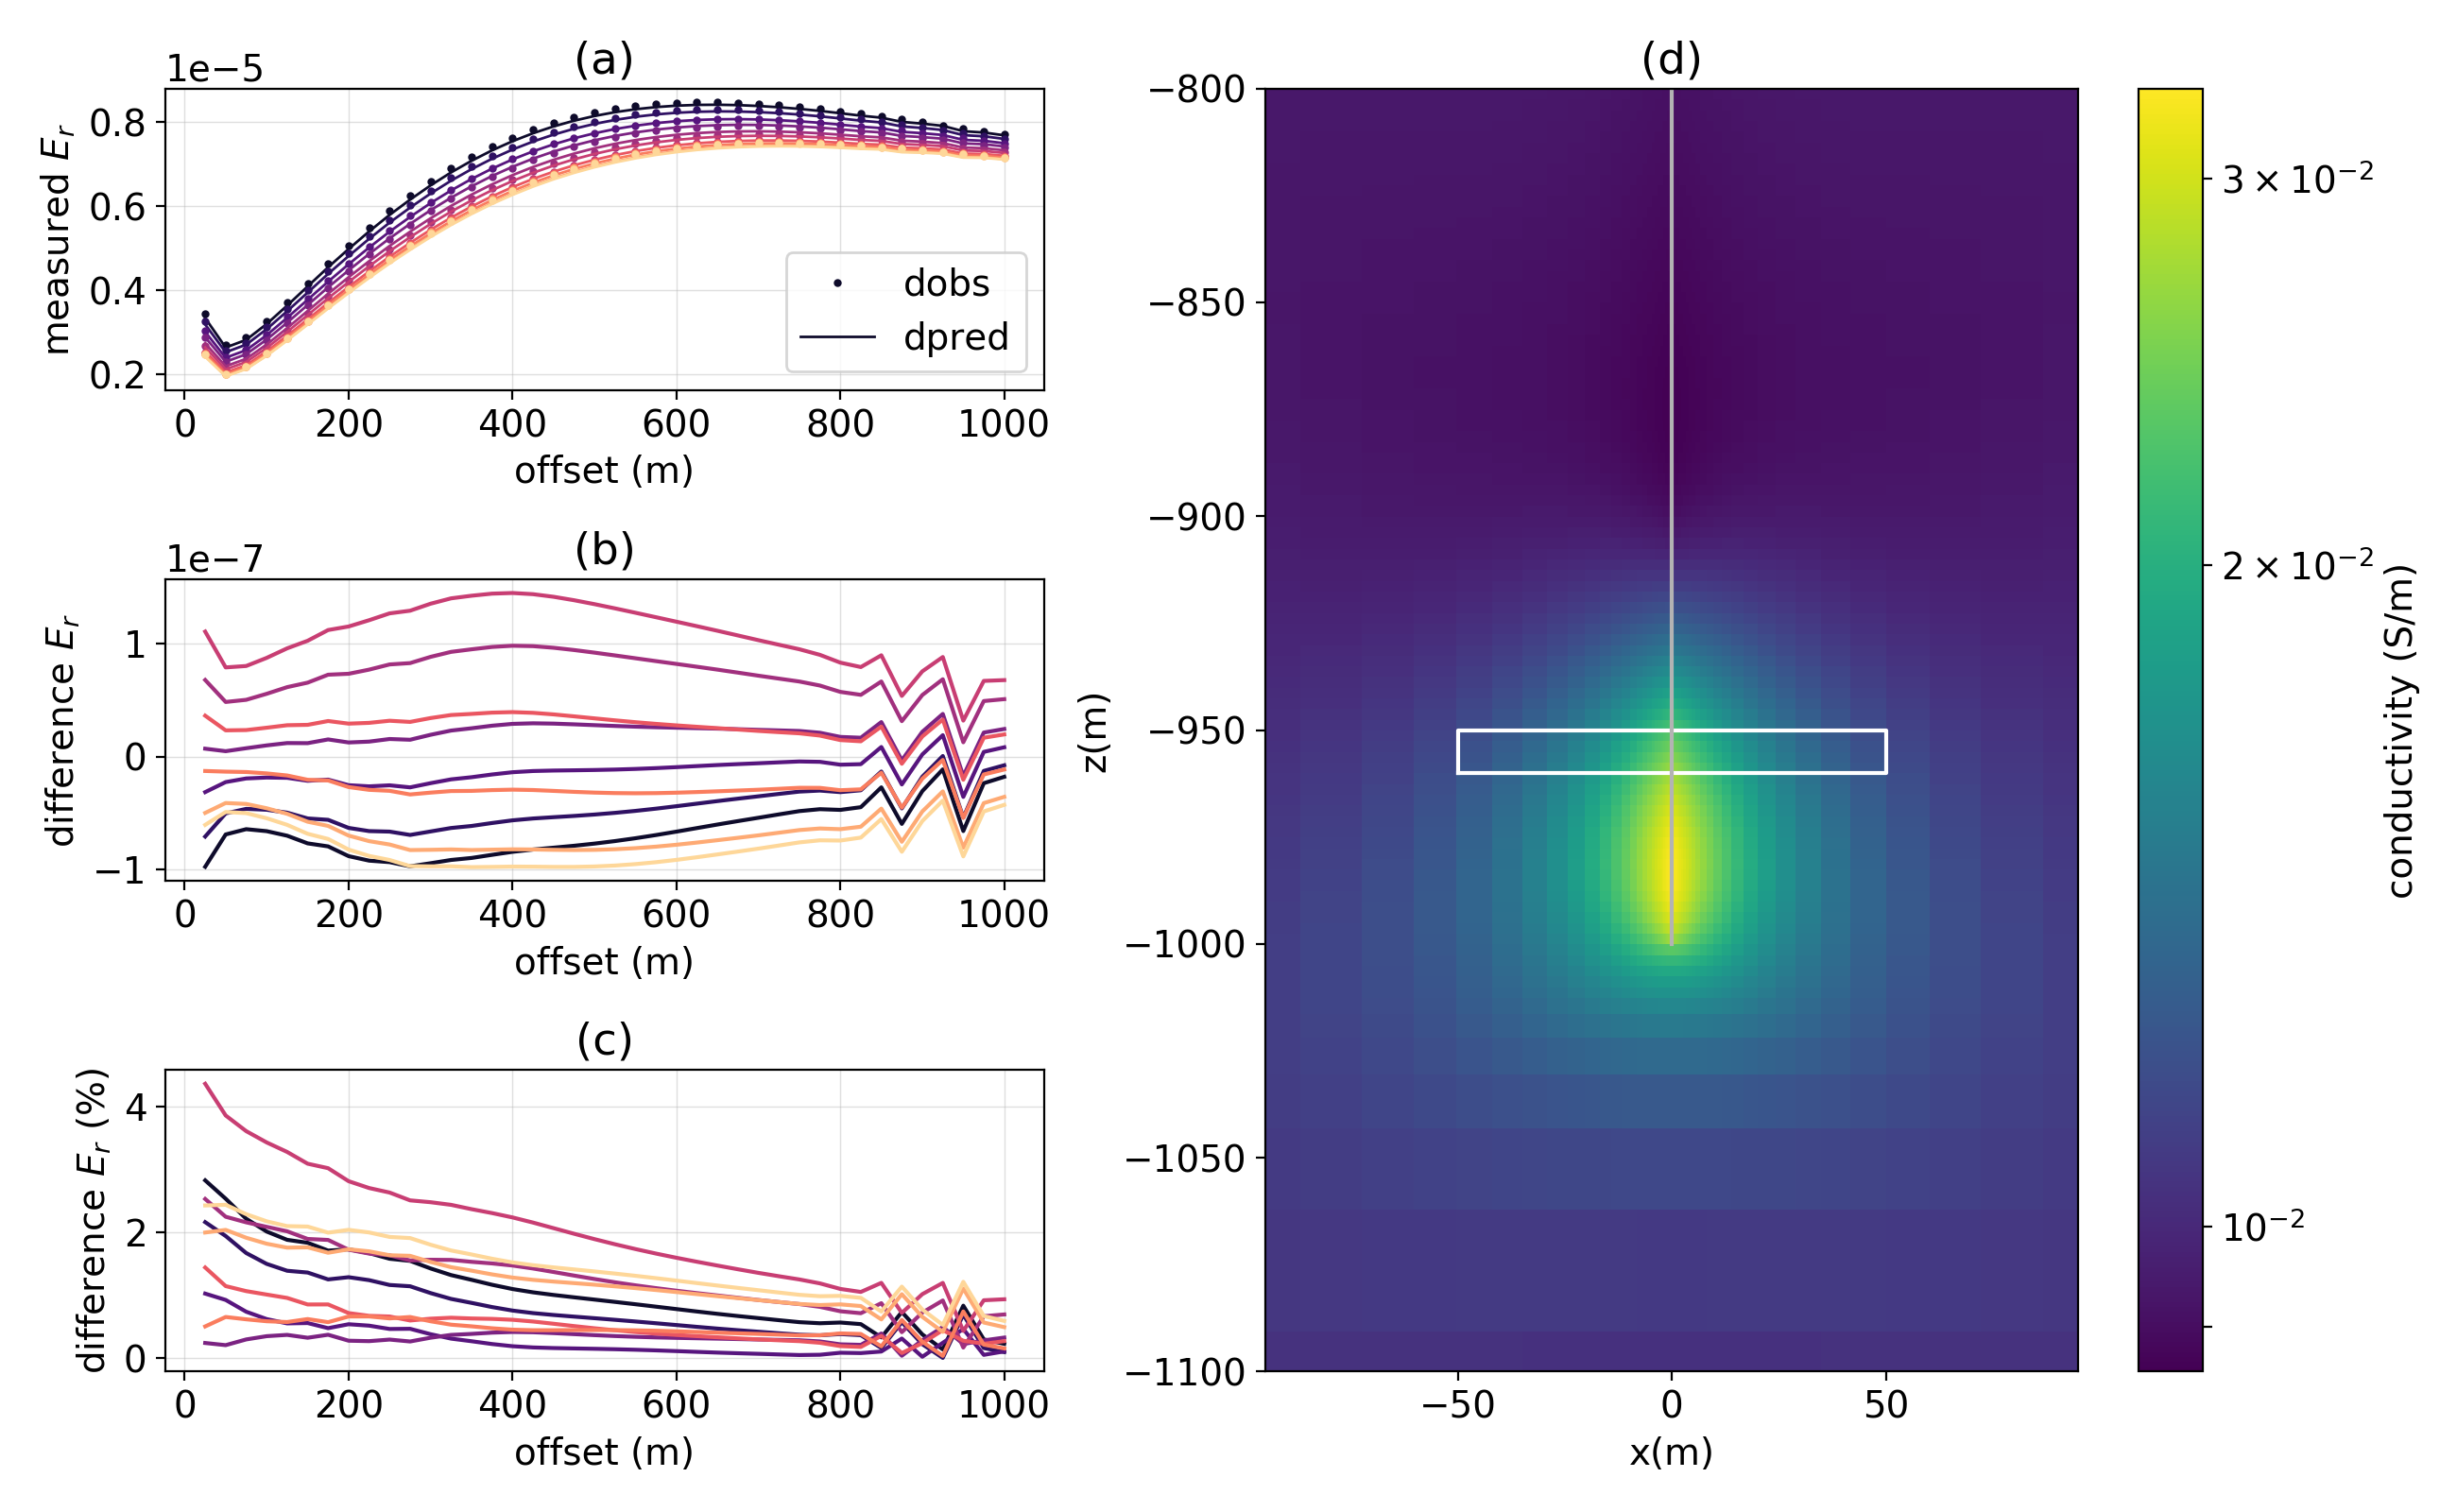
\includegraphics[width=1\textwidth]{figures/inversion/dc_smooth_inversion_1e-01.png}
    \end{center}
\caption{
    (a) Observed and predicted radial electric field data,
    (b) difference between the observed and predicted data (V/m),
    (c) difference between the observed and predicted data as a percentage of the observed data,
    and (d) conductivity model recovered in the inversion.
    The colors in (a), (b), and (c) indicate the source location as shown in Figure \ref{fig:dc_casing_initial_data}.
    The white outline in (d) outlines the true geometry of the fracture zone and the grey line shows the location of the wellbore.
    The data are fit to a global $\chi$-factor $<$ 0.1.
}
\label{fig:dc_smooth_inversion_1e-01}
\end{figure}




If we push the inversion harder, the depth of the target is better-resolved, as shown in Figure \ref{fig:dc_smooth_inversion_5e-02}. In practice, this requires very high data quality; here we fit all data points within $\sim2\%$ and reach a global $\chi$-factor $<$0.05. The geometry of the target that we recover is elongated vertically; this is consistent with having larger sensitivity near the well. We also notice that the conductivity of the background above the target drops beneath that of the background -- this is a common effect in smooth inversions when conductive targets are present. In this case, we know that the changes due to the conductive proppant and fluid should only increase the conductivity with respect to the background. We could impose a lower-bound on the conductivity of the inversion model, however, experimentation shows that this tends to push the center of the conductive anomaly beneath the true target depth.


\begin{figure}
    \begin{center}
    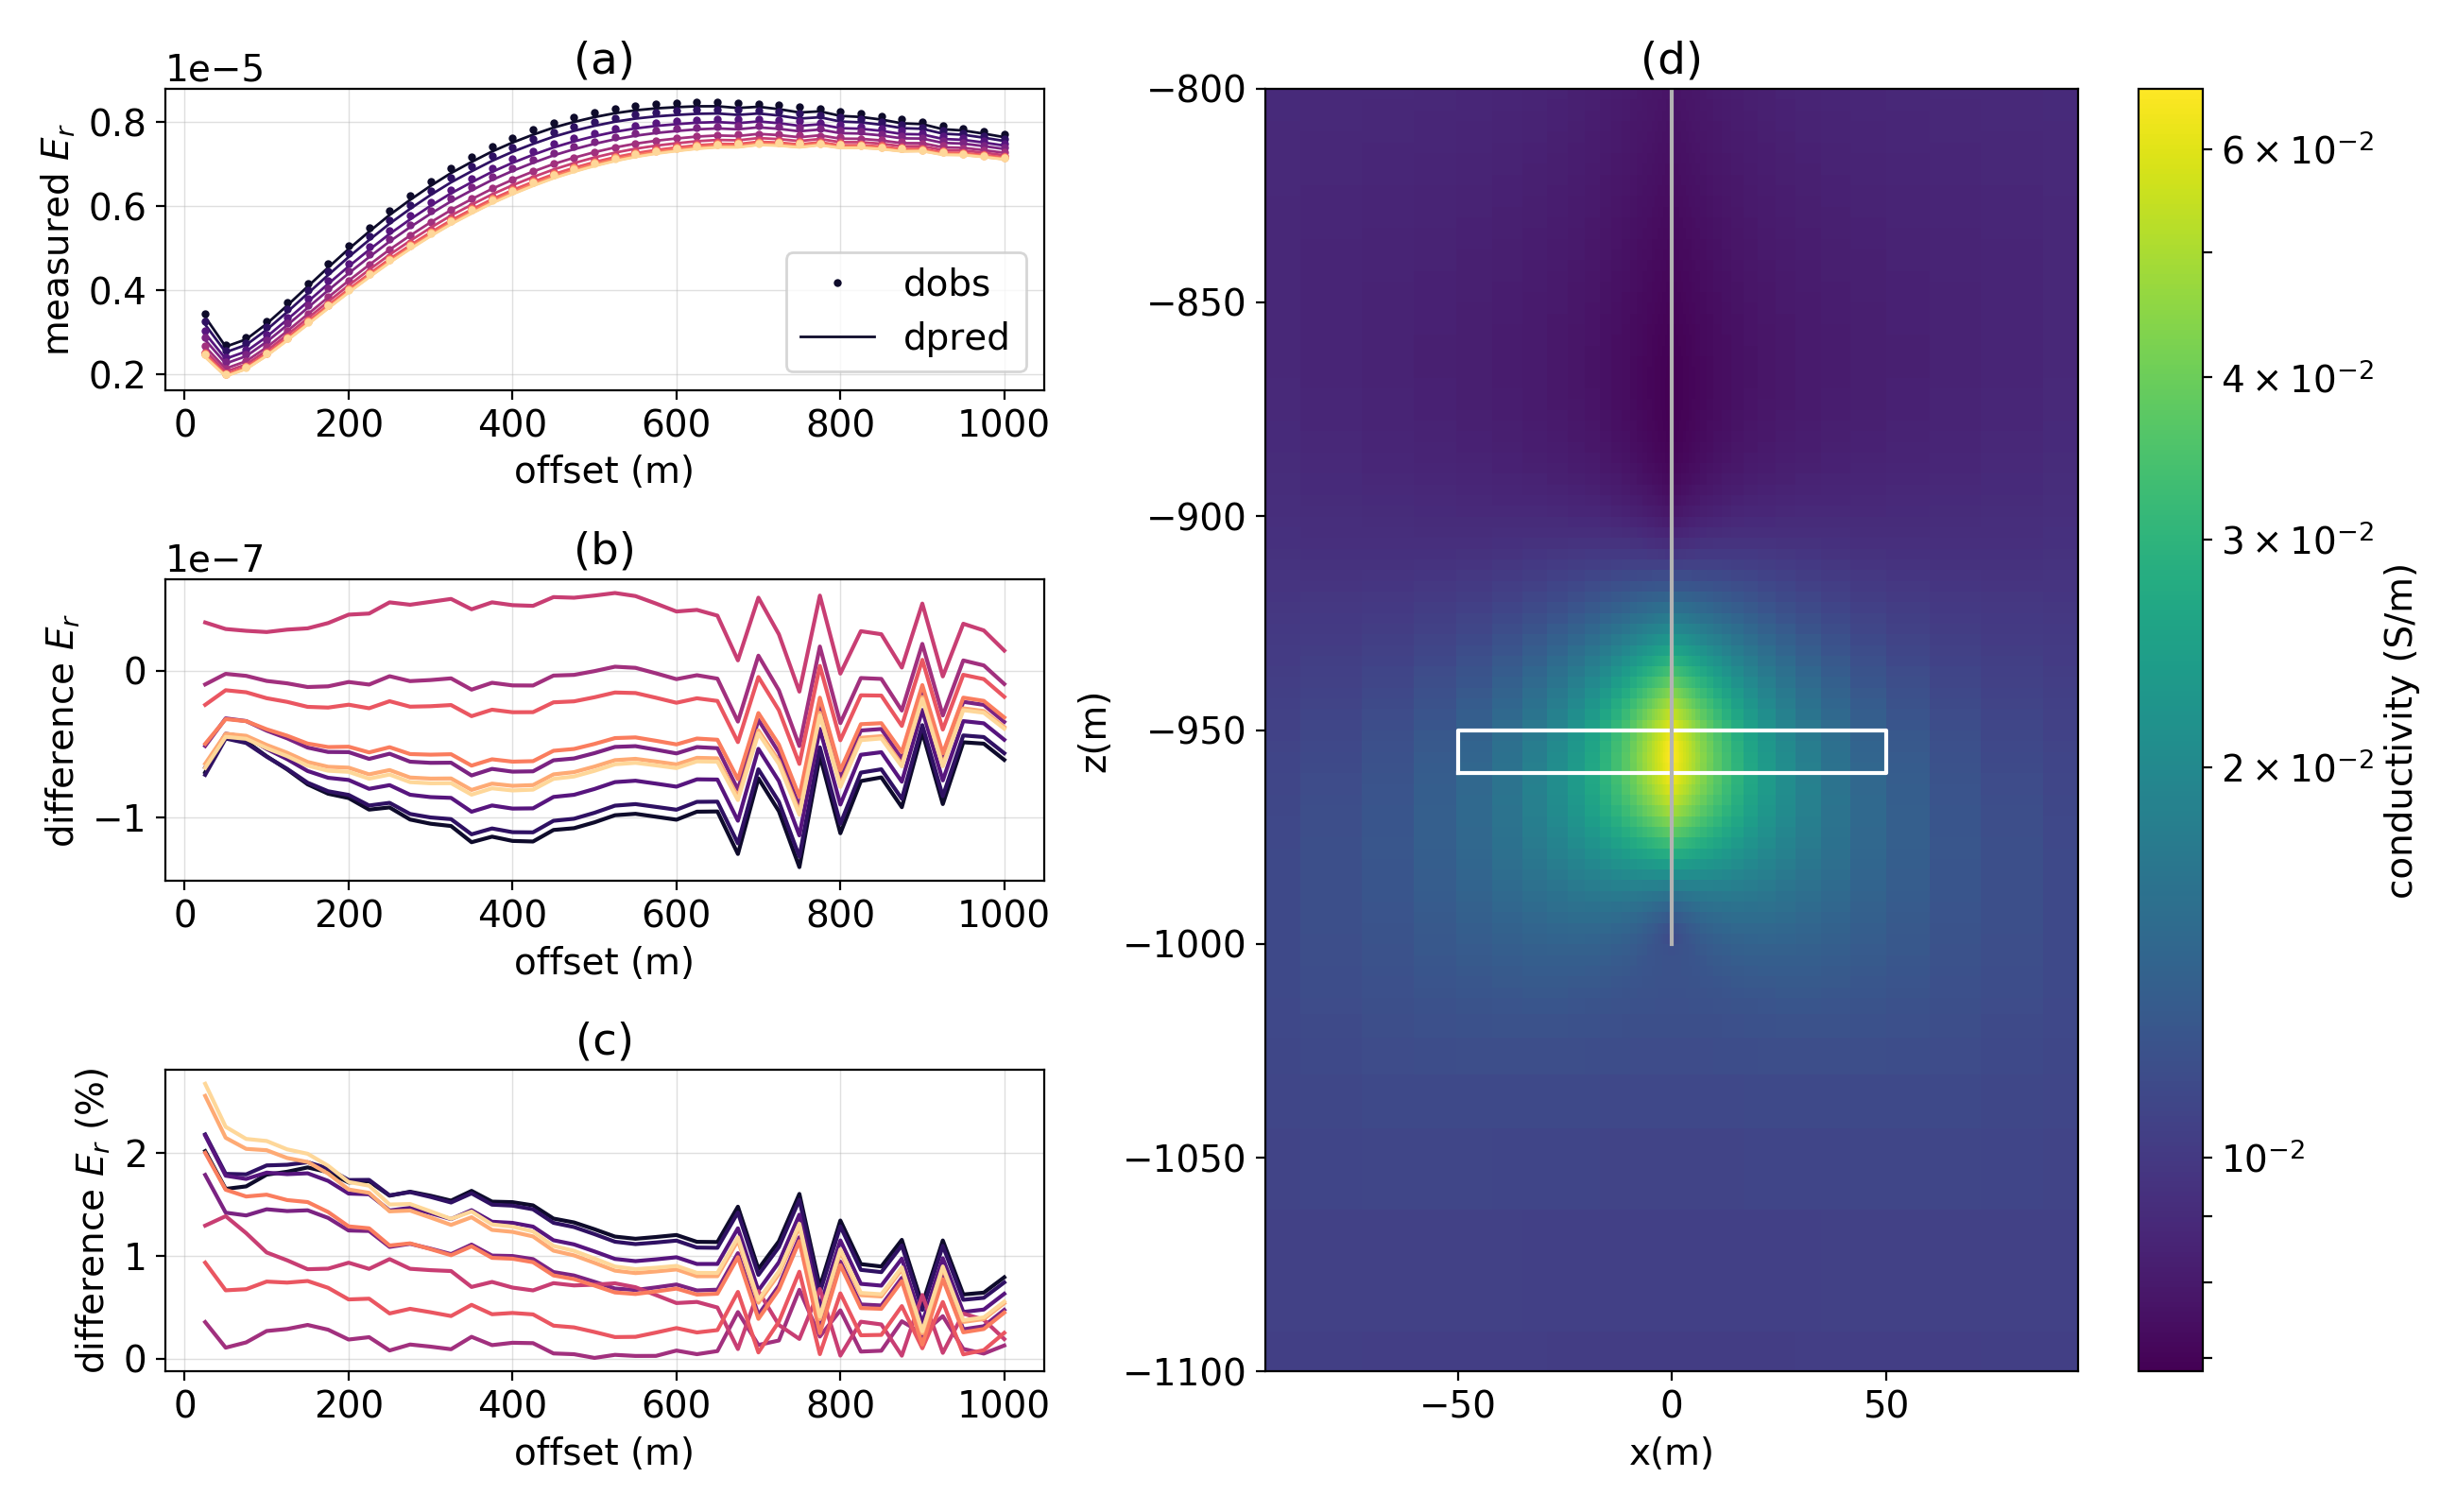
\includegraphics[width=1\textwidth]{figures/inversion/dc_smooth_inversion_5e-02.png}
    \end{center}
\caption{
    Tikhonov inversion result, similar to that shown in \ref{fig:dc_smooth_inversion_1e-01}
    that fits the data to a global $\chi$-factor $<$ 0.05.
}
\label{fig:dc_smooth_inversion_5e-02}
\end{figure}


To counter the vertical elongation of the target, we can always promote more horizontally elongated structures by altering the regularization. Figure \ref{fig:dc_smooth_inversion_5e-02_alpha_100} demonstrates an inversion using $\alpha_x=100$ and fitting the data to a $\chi$-factor $<$ 0.05. Using a large $\alpha_x$ smears out the target horizontally and also reduces the maximum conductivity as compared to Figure \ref{fig:dc_smooth_inversion_5e-02}.


\begin{figure}
    \begin{center}
    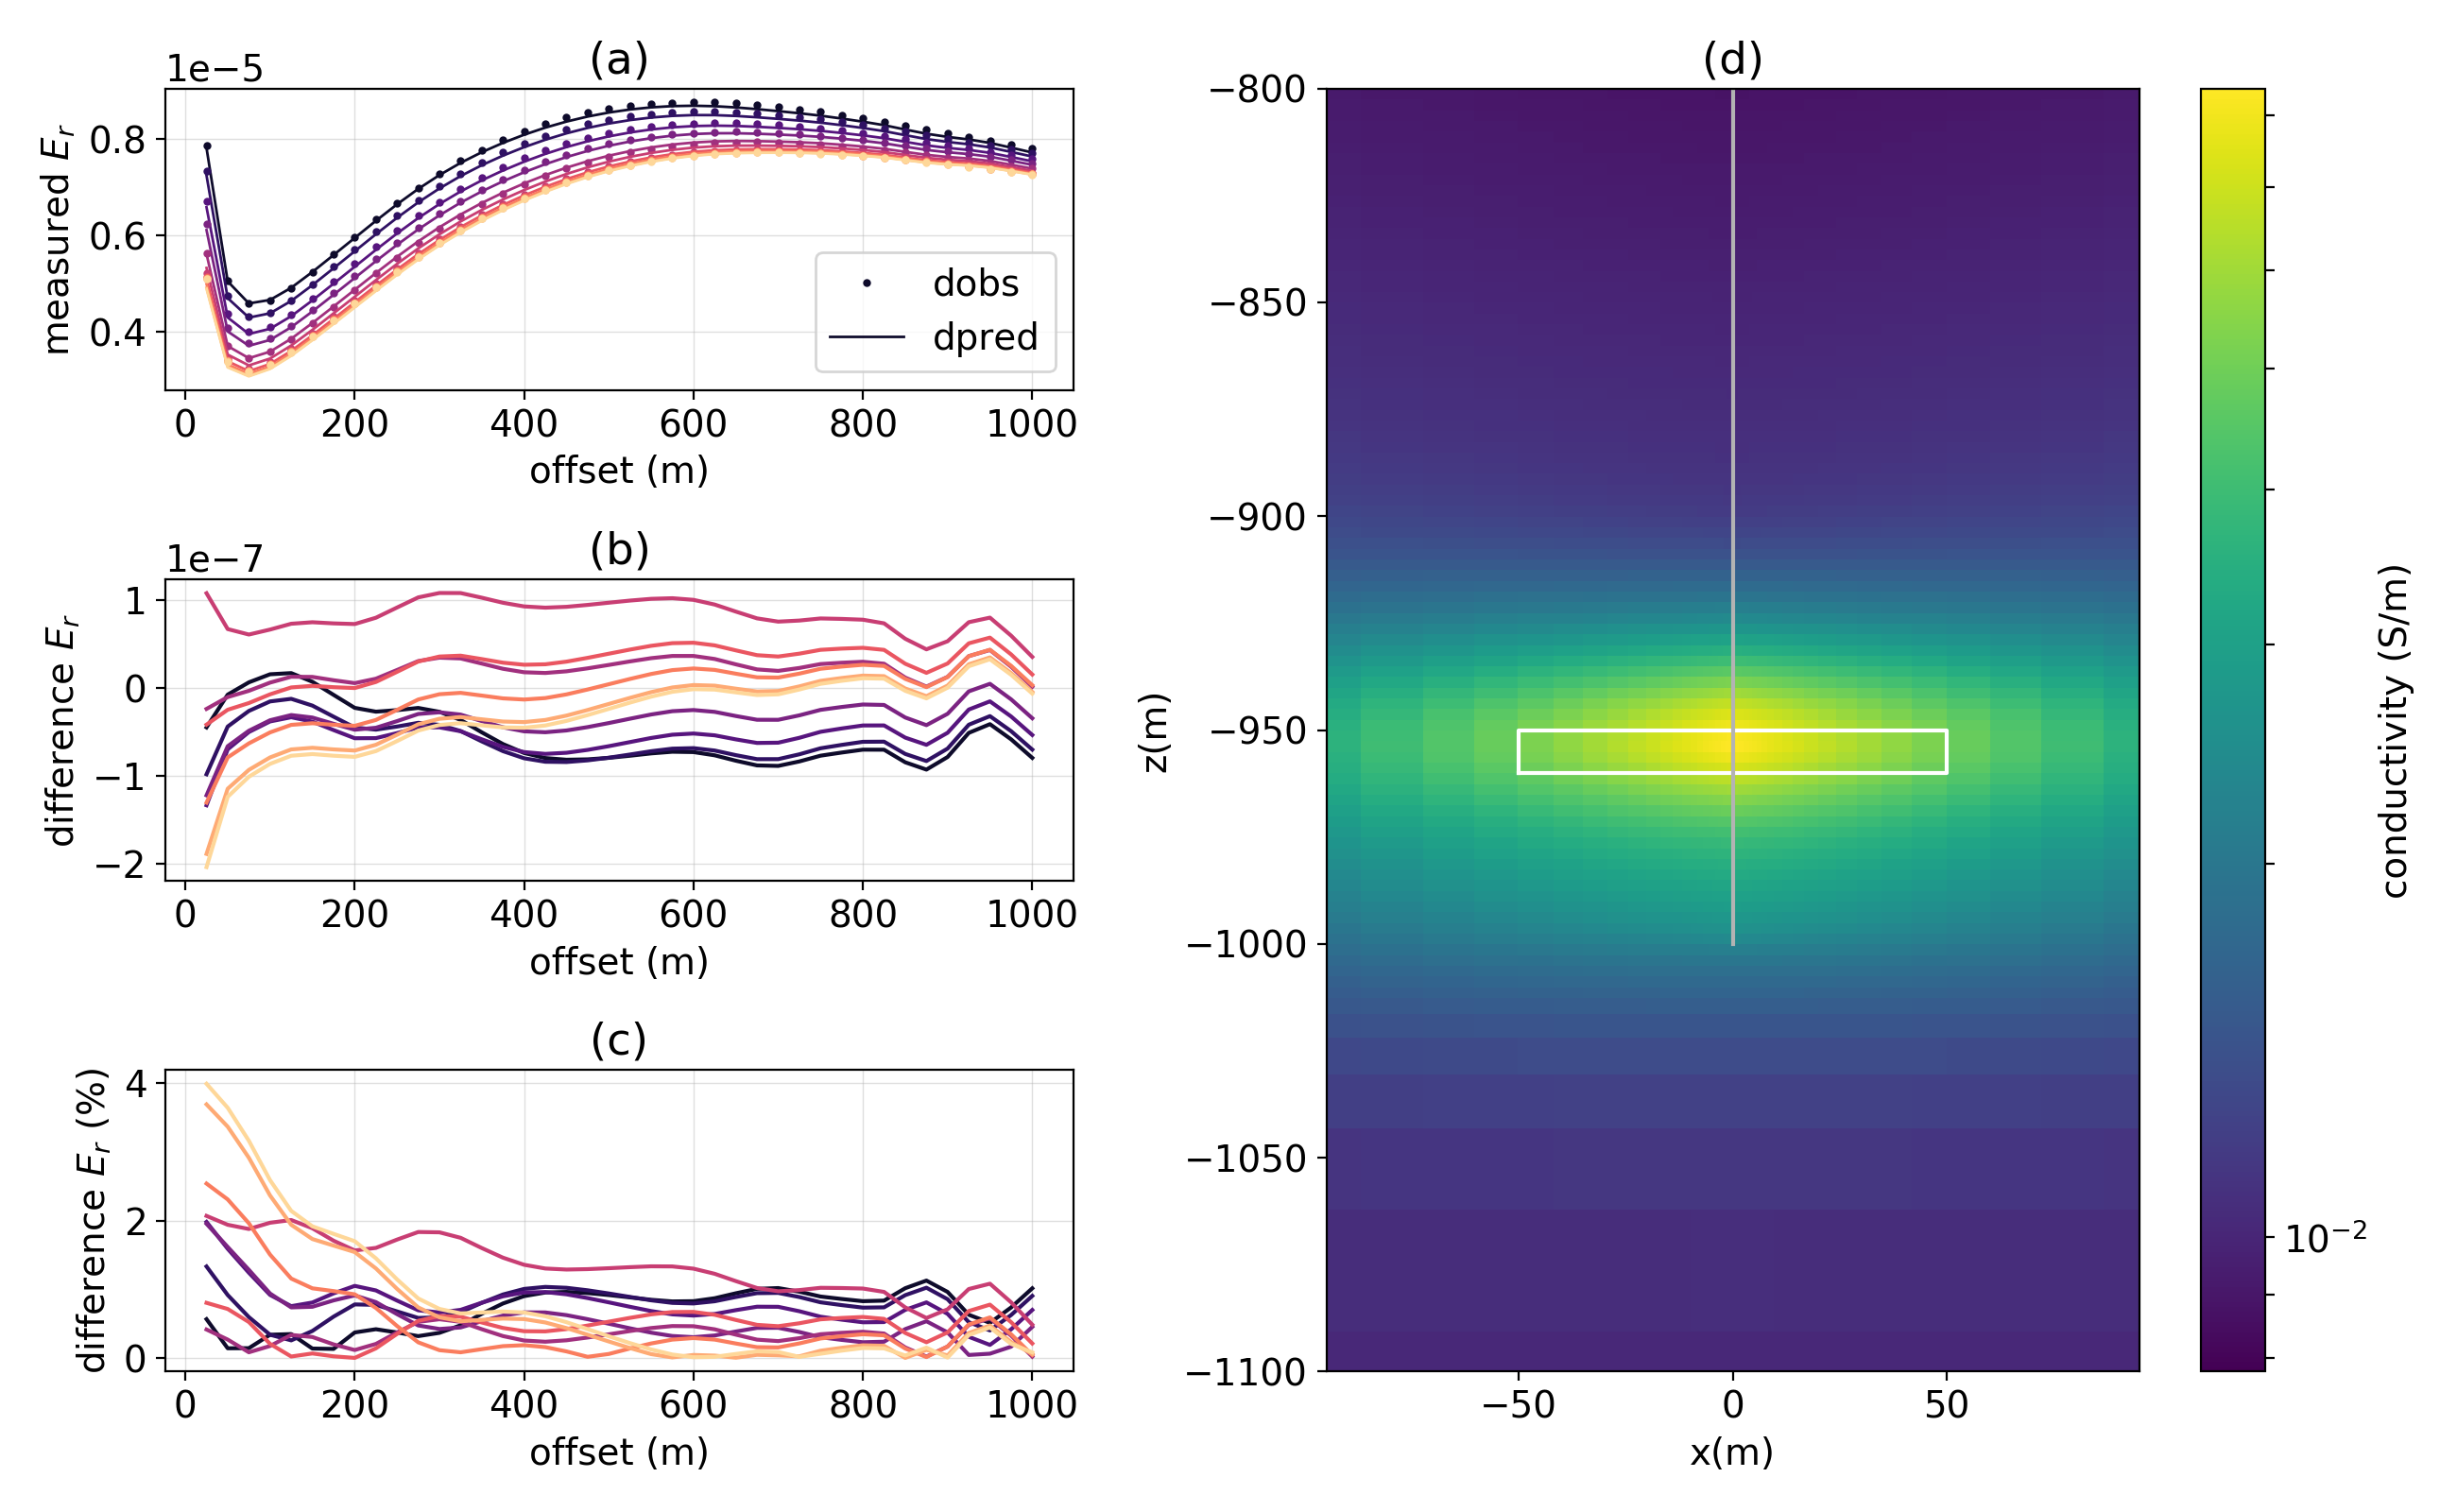
\includegraphics[width=0.8\textwidth]{figures/inversion/dc_smooth_inversion_5e-02_alpha_100.png}
    \end{center}
\caption{
    Tikhonov inversion result, similar to that shown in \ref{fig:dc_smooth_inversion_5e-02}
    that uses $\alpha_x = 100$. The inversion took 5 iterations.
}
\label{fig:dc_smooth_inversion_5e-02_alpha_100}
\end{figure}


Using a Tikhonov style inversion, we can recover a target at the correct location, and by adapting the $\alpha$ values, we can recover a general geometry reflective of the true target. However, these are not particularly insightful images for delineating the extent of the fractured region of the reservoir. With the aim of using the inversion to obtain parameters indicative of the injection, we next examine an approach using a parametric inversion.
\subsection{Parametric Inversion}
In a parametric approach to the inversion, we represent the fractured volume of rock as a simple geometric structure, and will invert for properties of the background, target and the position and geometry of the target. For the following examples, we treat the fractured volume of rock as a cylinder. We fix $x_0 = 0$m and invert for the log-conductivity of the background and the target, as well as the depth, radius and thickness of the target. We again push the inversion quite hard, fitting the following results to a global $\chi$-factor $<0.05$, meaning that most of the data are fit within $\sim 2\%$.

For the parametric inversion to find an initial step, it is important that we start with a model where target has physical properties distinct from the background. In this example, we build a starting model based on the first voxel inversion result, shown in Figure \ref{fig:dc_smooth_inversion_1e-01}. The center of the target is at 980m depth, its radius is 10m and it thickness is 5m. The conductivity of the background is $10^{-2}$ S/m and the conductivity of the target is set to $3 \times 10^-2$ S/m. Figure \ref{fig:parametric_voxel1} shows the recovered model; the true geometry is outlined by the solid white line and the starting model geometry is shown by the dashed white line. The depth and thickness of the recovered model are well-resolved. The radius is underestimated (18m) and the conductivity over-estimated (950 S/m).


\begin{figure}
    \begin{center}
    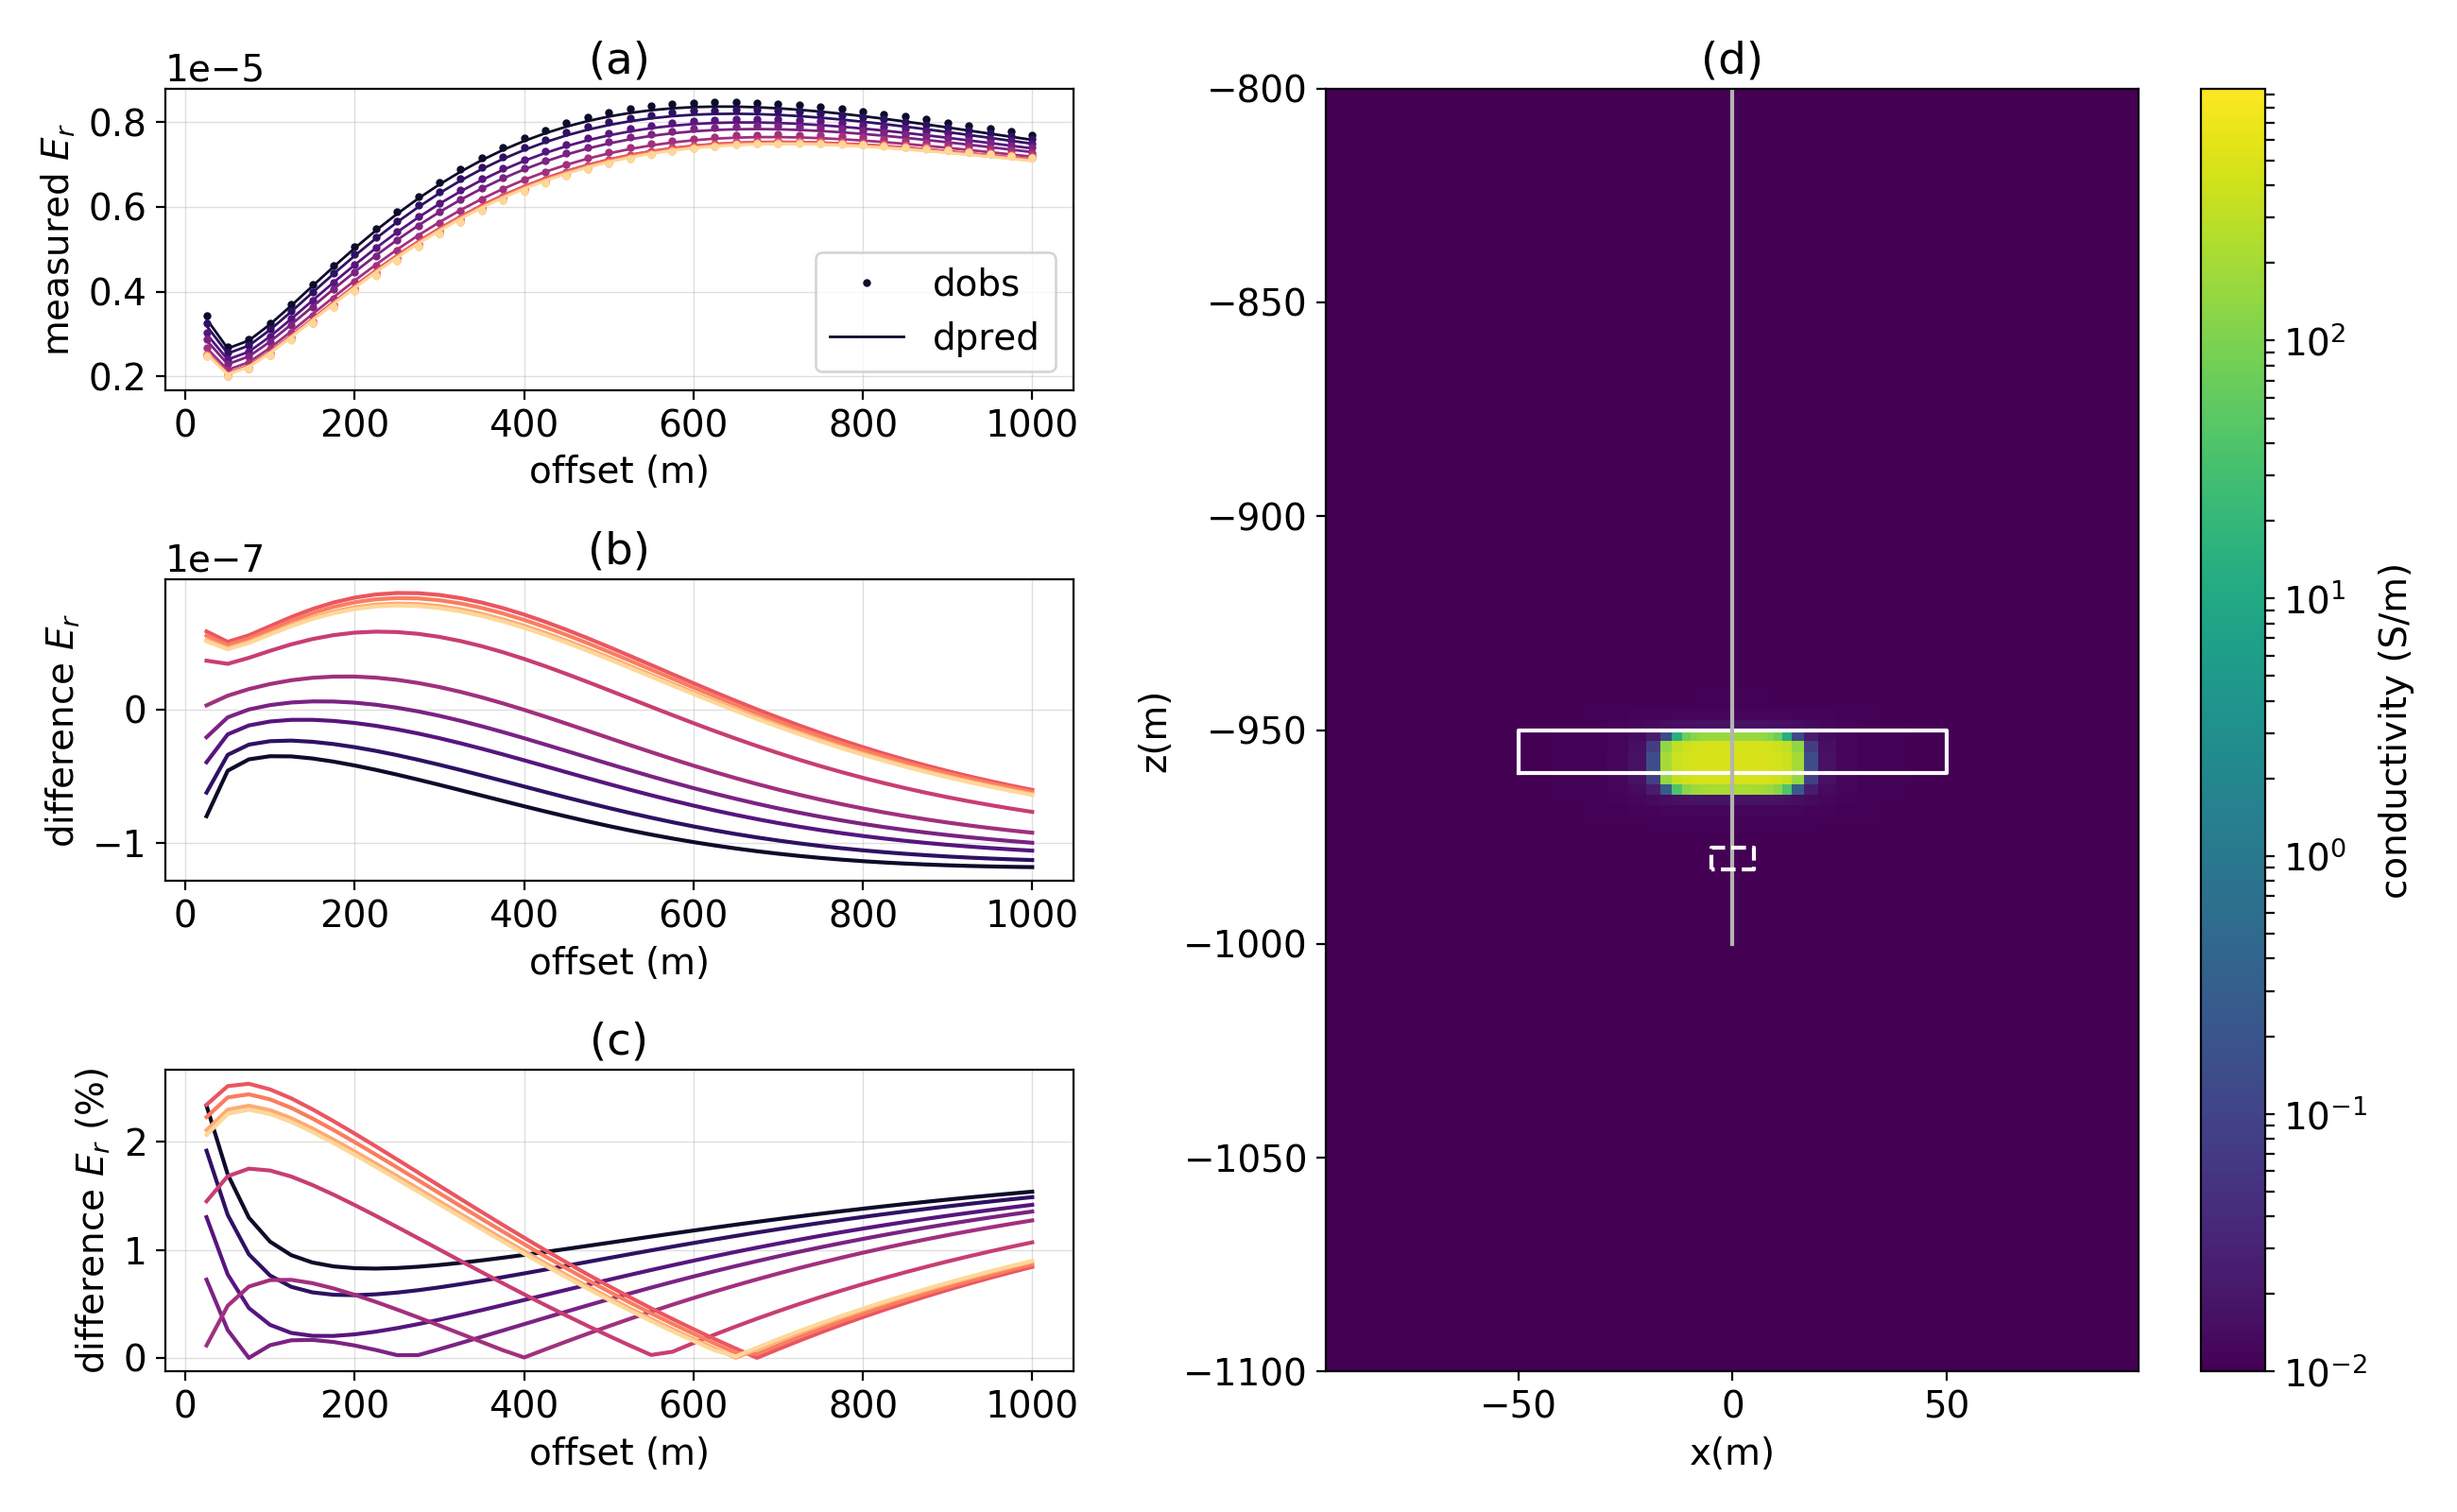
\includegraphics[width=1\textwidth]{figures/inversion/parametric_voxel1.png}
    \end{center}
\caption{
    Parametric inversion result for a starting model
    centered at 980m depth with a thickness of 5m and a radius of 10m. The initial background
    conductivity is $10^{-2}$ S/m and the initial conductivity of the target is $3\times10^{-2}$ S/m.
    The geometry of the starting model is shown by the white dashed-lines and the
    true model is shown by the solid white outline. The inversion reached a $\chi$-factor < 0.05
    and took 8 iterations.
\label{fig:parametric_voxel1}
\end{figure}


If instead, we use the true depth-center of the target, informed by the inversion result in Figure \ref{fig:dc_smooth_inversion_5e-02}, we obtain the model shown in Figure \ref{fig:parametric_voxel2}. The starting conductivities, radius and thickness were the same used in the previous inversion. Here, the depth to the center of the target remains at the correct location, and the recovered radius, 55m, is closer to the true model. However, the recovered conductivity, $10^9$ S/m is drastically over-estimated. Typically, one might expect that there is a saturation in the conductivity effects for a DC experiment. For example, if we consider a conductive sphere in a half-space, whether the conductivity of the sphere is 2 or 3 orders of magnitude larger than the background, makes little difference in the data. However, in this example, the conductive target is directly coupled to the casing, which has a conductivity of $10^4$ S/m. We suspect that this survey geometry is sensitive to a larger dynamic range of conductivity values and this might contribute to the large updates in the electrical conductivity of the target.

\begin{figure}
    \begin{center}
    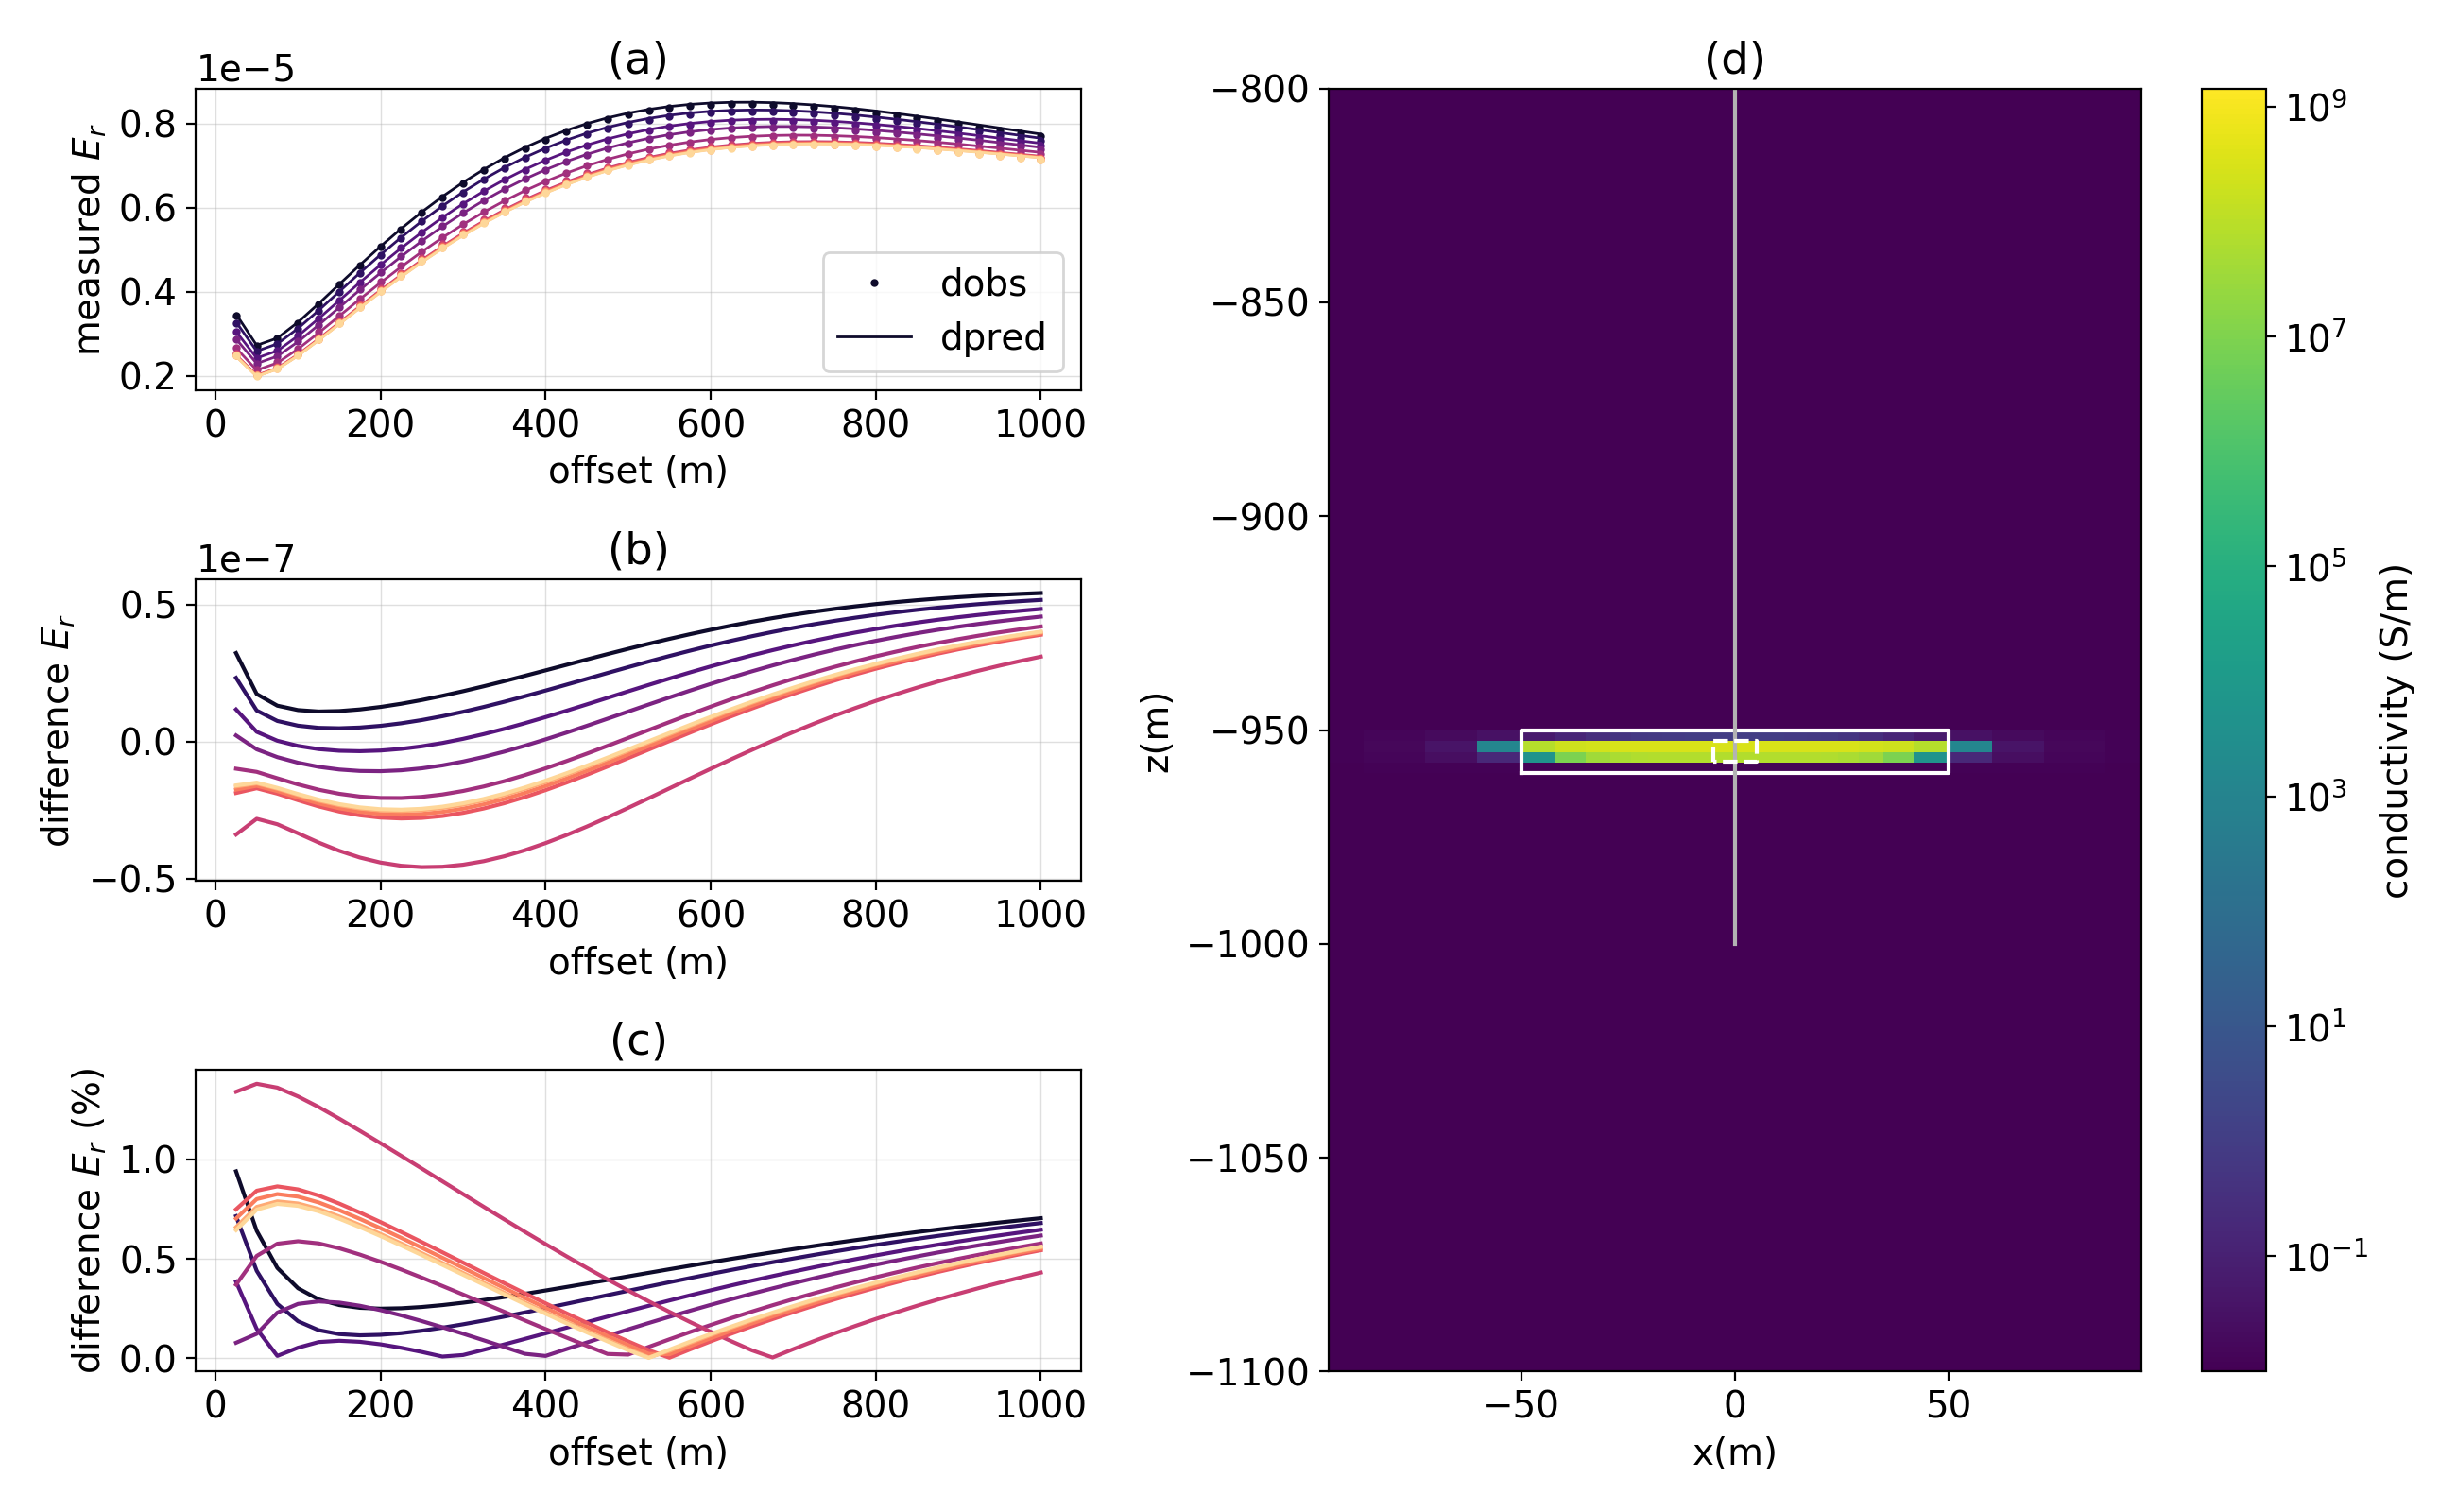
\includegraphics[width=0.8\textwidth]{figures/inversion/parametric_voxel2.png}
    \end{center}
\caption{
    Parametric inversion result for a starting model
    centered at 955m depth with a thickness of 5m and a radius of 5m. The initial background
    conductivity is $10^{-2}$ S/m and the initial conductivity of the target is $3\times10^{-2}$ S/m.
    The geometry of the starting model is shown by the white dashed-lines and the
    true model is shown by the solid white outline. The inversion reached a $\chi$-factor $<$ 0.05
    and took 8 iterations.
}
\label{fig:parametric_voxel2}
\end{figure}


The casing spreads out the source currents along its length, this may reduce sensitivity to the depth and thickness of the target. If that is the case, perhaps starting with the correct depth-center and thickness will improve the result. Figure \ref{fig:parametric_voxel2_dz10} shows the recovered model when the correct depth and vertical extent of the target are used for the starting model. The conductivity is still over-estimated (960 S/m), but not nearly as severe as the previous inversion. The depth has been shifted down beneath the target, and the radius (23 m) is underestimated.


\begin{figure}
    \begin{center}
    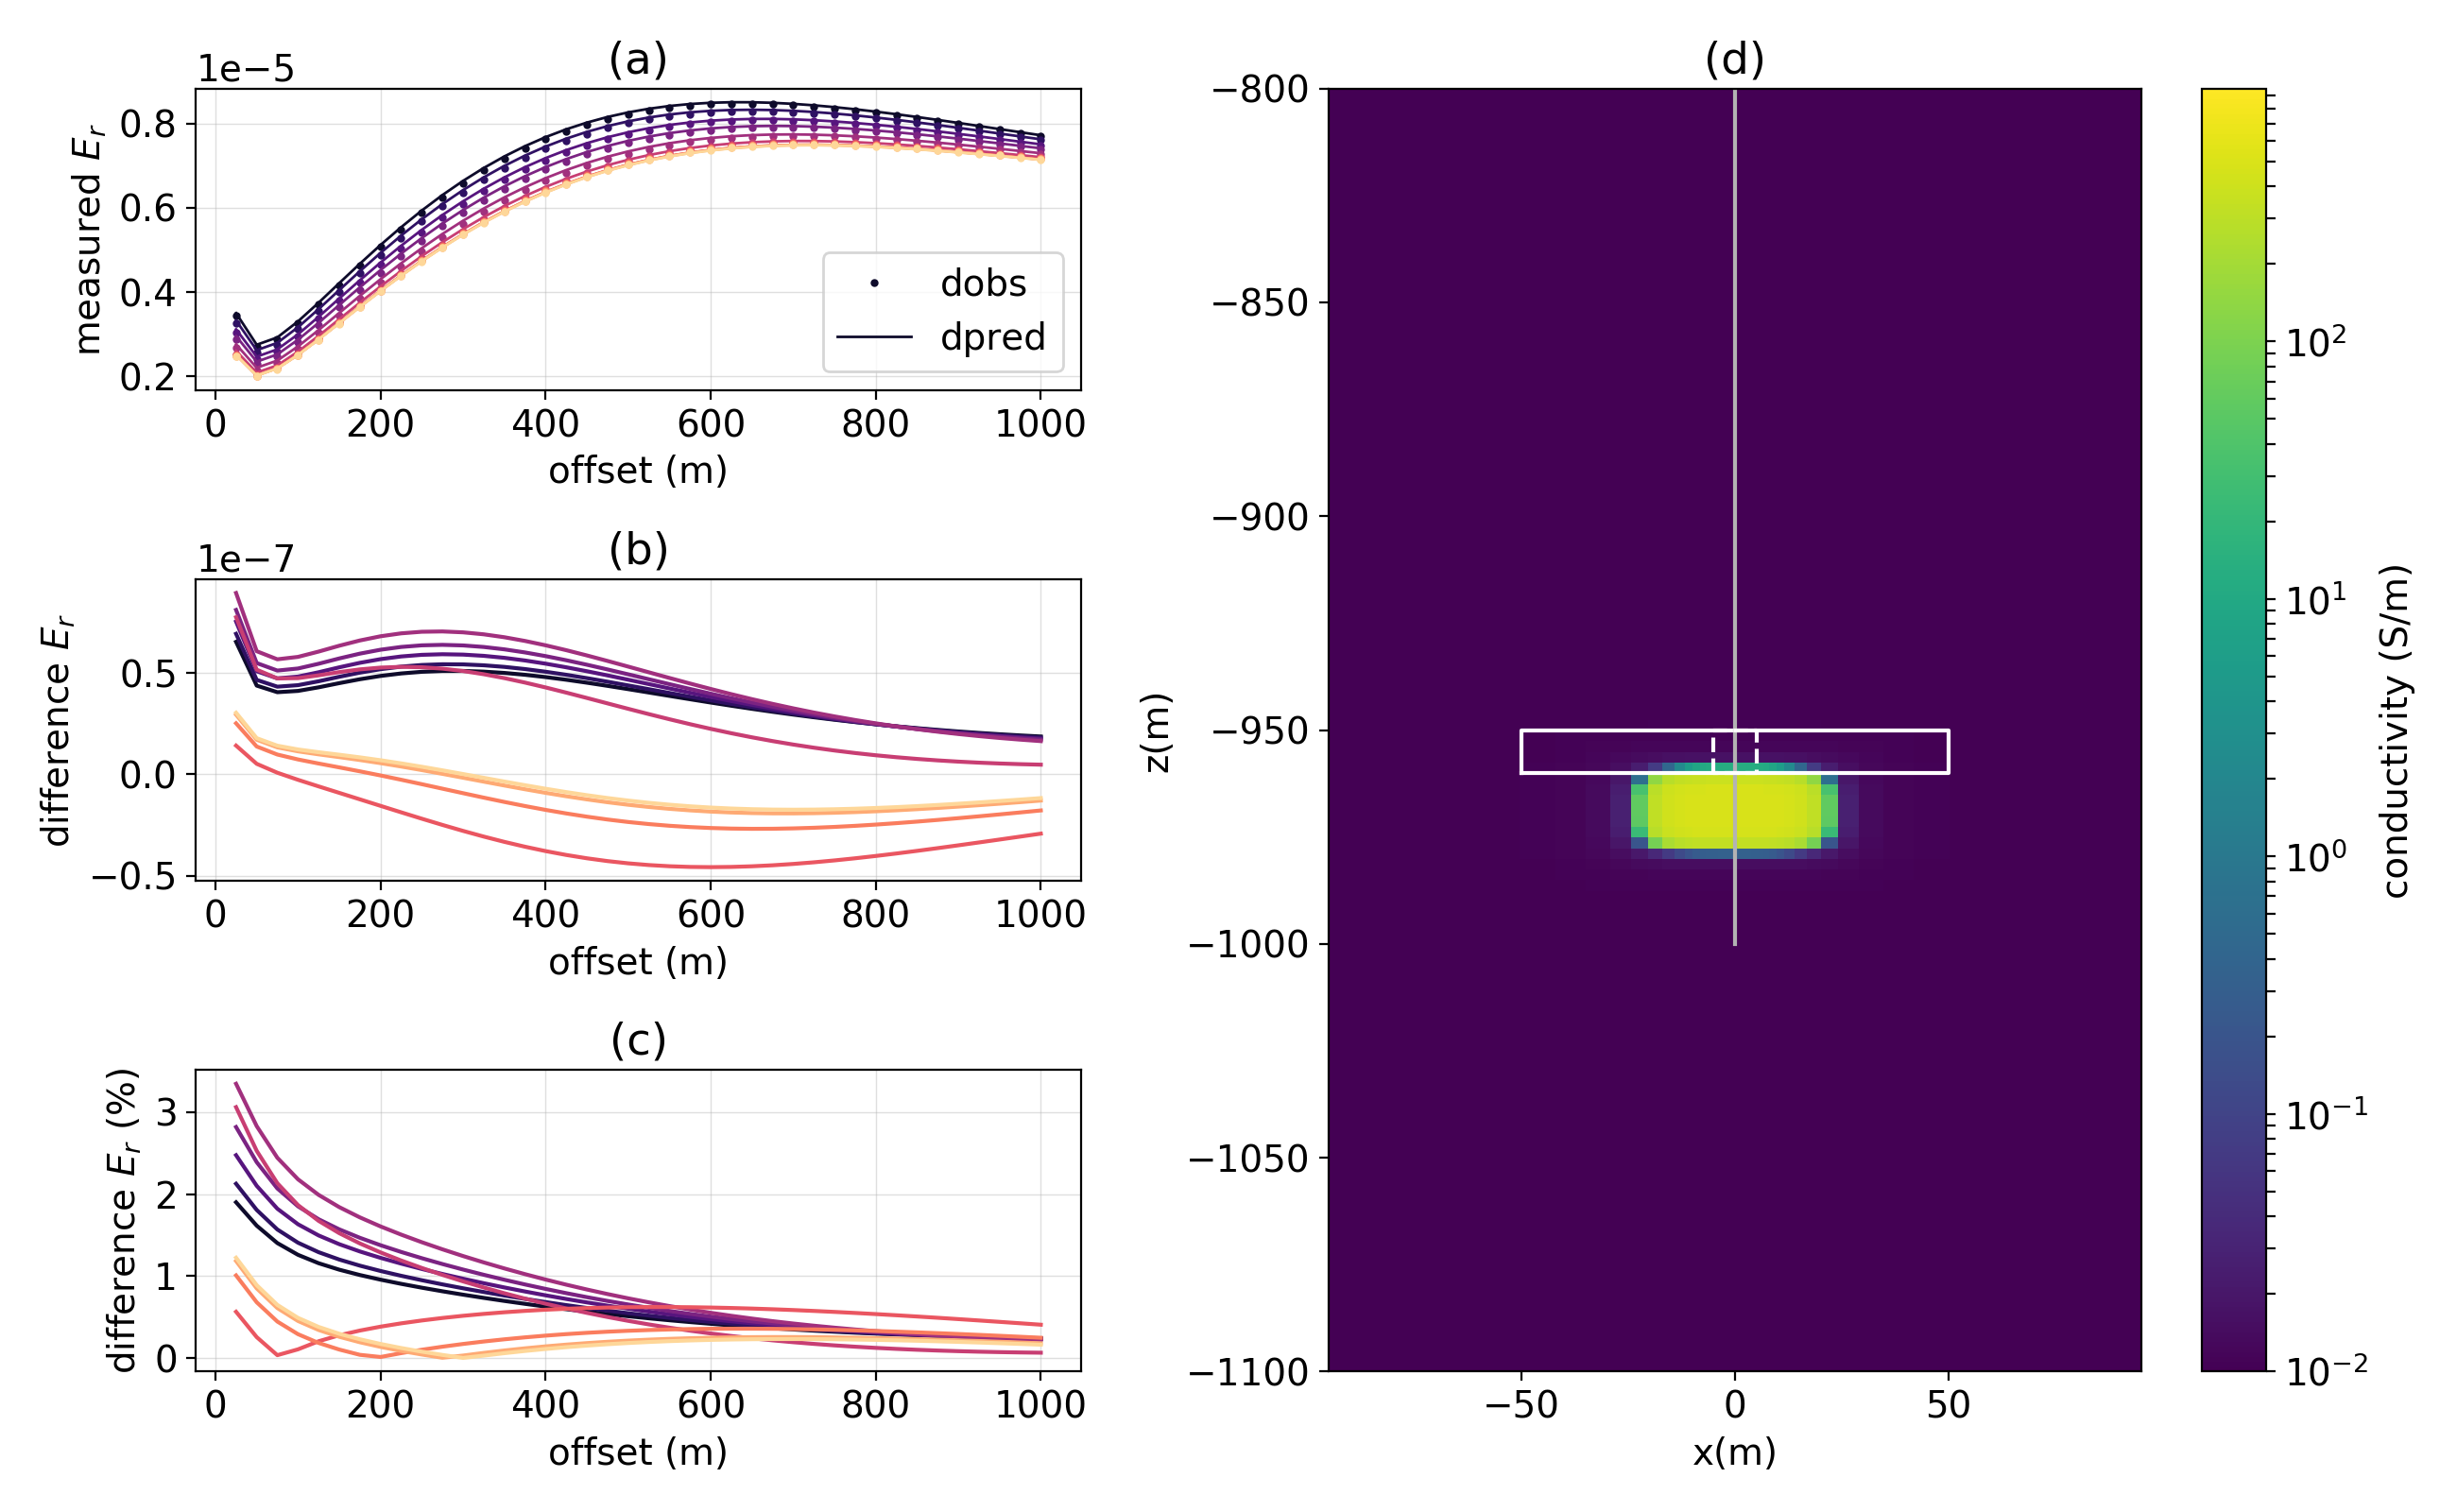
\includegraphics[width=1\textwidth]{figures/inversion/parametric_voxel2_dz10.png}
    \end{center}
\caption{
    Parametric inversion result for a starting model
    centered at 955m depth with a thickness of 10m and a radius of 10m. The initial background
    conductivity is $10^{-2}$ S/m and the initial conductivity of the target is $3\times10^{-2}$ S/m.
    The geometry of the starting model is shown by the white dashed-lines and the
    true model is shown by the solid white outline. The inversion reached a $\chi$-factor < 0.05
    and took 8 iterations.
\label{fig:parametric_voxel2_dz10}
\end{figure}


Presumably, the injection point is known, and therefore it might be reasonable to fix the value of $z_0$ in the inversion. In Figure \ref{fig:parametric_voxel2_dz10_fixedz0}, we have run an inversion using the same starting model as in the previous inversion, but now have fixed the location of the target to the true target depth of 955m depth. The radius of the recovered model is very similar to that shown in Figure \ref{fig:parametric_voxel2_dz10}, as is the thickness (25 m). The conductivity, $0.7$ S/m, much closer to the true conductivity (3 S/m) than any of the previous inversions.


\begin{figure}
    \begin{center}
    \includegraphics[width=1\textwidth]{figures/inversion/parametric_fixed_z0.png}
    \end{center}
\caption{
    Parametric inversion result where the center of the target is fixed at a depth
    of 955m. The starting model has a thickness of 10m and a radius of 10m. The initial background
    conductivity is $10^{-2}$ S/m and the initial conductivity of the target is $3\times10^{-2}$ S/m.
    The geometry of the starting model is shown by the white dashed-lines and the
    true model is shown by the solid white outline. The inversion reached a $\chi$-factor < 0.05
    and took 7 iterations.
\label{fig:parametric_fixed_z0}
\end{figure}



